\documentclass{scrartcl}
    \usepackage[utf8]{inputenc}
    \usepackage[T1]{fontenc}
    \usepackage[naustrian]{babel}
    \usepackage{scrextend}
    \usepackage{enumerate}
    \usepackage{graphicx}
    \usepackage{verbatim}
  

    \title{Rechnernetze \& Netzwerkprogrammierung - VO-Vorbereitung}
    \author{T. Auer, C. Bauer} % Add your own shithole
    \date{Latest Update: \today}
    
% ----------------------------------------------------------------------------------------------
% 1. If you add something, add yourself to Authors. Also, Update changes & TODOs. 
% 2. Shared file is shared. No Limits.
%       Use 'https://de.sharelatex.com/read/vknswmnmcgyv' to share file.
%       !!! DO NOT USE THE LINK GIVEN TO YOU. It gives Write-permissions apart from viewing doc.
% 3. Call in Discord before doing remarkable changes.
% 4. Don't write everything & consider the important shitholes first.
% -----------------------------------------------------------------------------------------------
% V.0.00.0013
%   Latest Changes:     * Additional Questions from the test.
%               
%   TODOS:              * More Theory
%                       * Java Impls ?
%                       * Formatting. Some things are flushing wildly
%                       * Some Items are missing here and there.
% -----------------------------------------------------------------------------
    
\begin{document}
\maketitle
\hrulefill
\tableofcontents
\hrulefill
\newpage
    
\section{ISO/OSI-Referenzmodell vs TCP-IP}
    \begin{center}
        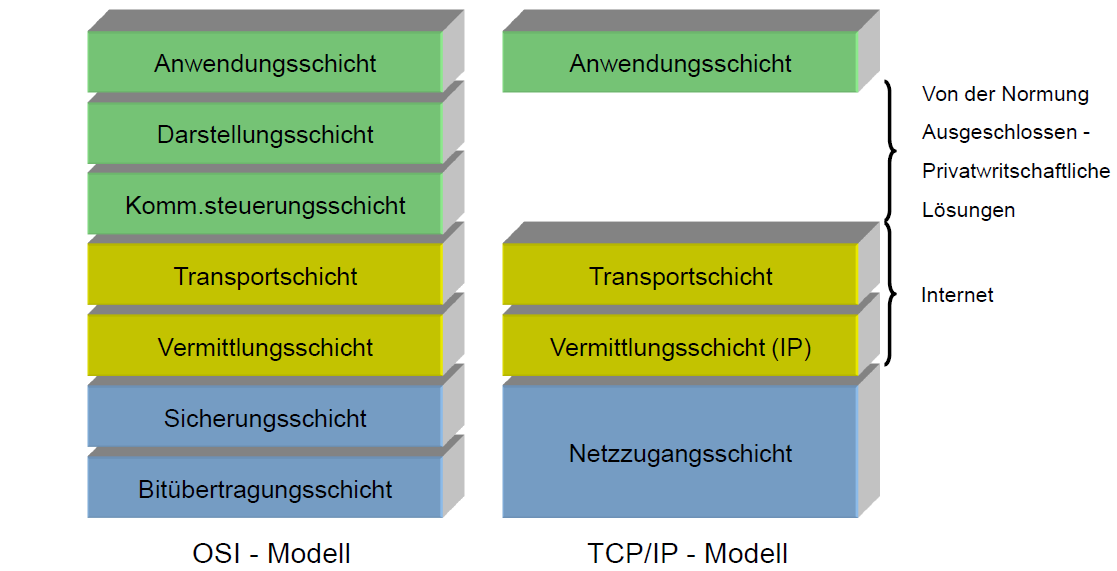
\includegraphics[width=\textwidth]{tcp_ip_model.png}
    \end{center}
    \subsection{OSI-Modell}
    \subsubsection{Application Layer}
    \label{OSI:application_layer}
    Im OSI-Modell dient der Application Layer dem Userinterface. Es handled I/O, bietet Userfunktionen und initiiert Verbindungen zu unterliegenden Schichten.
    Bsp.: Webbrowser, E-Mail Dienste, Instant Messaging.
    \paragraph{Protokolle:}
    \begin{itemize}
        \item HTTP,
        \item DNS,
        \item BGP, 
        \item SMTP, 
        \item POP3,
        \item IMAP.
    \end{itemize}
    \subsubsection{Presentation Layer}
    \label{OSI:presentation_layer}
    Wandelt systemabhängige Daten (ASCII, EBCDIC) in systemunabhängige Datenformate (ASN.1) um oder behandelt Datenkompression und Verschlüsselung.
    
    \paragraph{Protokolle:}
    \begin{itemize}
        \item Telnet,
        \item Tox,
        \item Network Data Representation,
        \item NetWare Core Protocol.
    \end{itemize}

    \subsubsection{Session Layer}
    \label{OSI:session_layer}
    Steuert Verbindungen in Form von Prozesskommunikation zweier Systeme, zum Datenaustausch. 
    Es handelt sich hierbei um einen semi-permanenten Dialog bestehend aus Anfragen und Antworten.

    \paragraph{Hauptfunktionalitäten:}
    \begin{itemize}
        \item Authentifizierung,
        \item Session Restoration.
    \end{itemize}

    \paragraph{Protokolle:}
    \begin{itemize}
        \item Rmote Procedure Call Protocol,
        \item Point-to-Point Tunelling Protocol,
        \item Real-Time Transport Control Protocol, 
        \item Session Control Protocol.
    \end{itemize}

    \subsubsection{Transport Layer}
    \label{OSI:transport_layer}
    In TCP/IP als auch im OSI-Modell: Realisiert Verbindung zwischen Quell-, und Zielhost mittels TCP und UDP. 
    Es dient dem Zuordnen von Datenpaketen zu einer spezifischen Anwendung.
    \begin{center}
        \begin{tabular}{l|l}
        \textbf{TCP} & \textbf{UDP}             \\\hline
        Congestion Control  &   Best Effort     \\
        Flow Control        &   Fast            \\
        'Handshake'         &   Low Overhead    \\
        Full-Duplex Data    &   Multicast       \\
        Connection-oriented &   Connectionless  \\
        Point-to-Point      &   Point-to-X      \\
        Reliable stream     &   Unreliable      \\
        Pipelined           &                   \\
    \end{tabular}
    \end{center}
    Weitere Protokolle:
    \begin{description}
        \item [SCTP] -- Stream Control Transmission Protocol,
        \item [TLS] -- Transport Layer Security: TCP + Verschlüsselung,
        \item [DTLS] -- Datagram Transport Layer Security: TLS + UDP.
    \end{description}

    \subsubsection{Network Layer}
    \label{OSI:network_layer}
    Implementiert Internet Protocol, IP. Die Zustellung der Daten zum richtigen Empfänger ist die Aufgabe von IP, e.g. das Routing, in sowohl leitungsorientierten als auch paketorientierten Verbindungen. 
    Zudem das Bereitstellen netzwerkübergreifender Adressen, Aktualisierung von Routingtabellen und Fragmentierung von Datenpaketen. 
    \begin{description}
        \item [IP] -- Internet Protocol: Übertragung,
        \item [IPsec] -- Internet Protocol Security: Sichere Datenverbindung,
        \item [ICMP] -- Internet Control Message Protocol: Kontrollnachrichten, Teil jeder IP,
        \item [OSPF] -- Open Shortest Path First: Informationsaustausch zwischen Routern,
        \item [BGP] -- Border Gateway Protocol: Informationsaustausch zwischen autonomen Systemen,
        \item [IGMP] -- Internet Group Management: Definiert Multicast-Gruppen.
          
        \end{description}

        

    \subsubsection{Data Link Layer}
    \label{OSI:data_link_layer}
    Segmentiert Pakete in Frames und checkt Prüfsummen. 
    Man prüft die fehlerfreie Übertragung als auch Zugriff auf Übertragungsmedium, 
    Bridge und/oder Switch. Nach IEEE ist sie in Logical Link Control und MAC aufgeteilt (In der VO: Data Plane, Control Plane). 
    
    \begin{enumerate}
        \item ARP - IPv4 Adressierung in Ethernet-Netzwerken (IPv6 -- NDP),
        \item Shortest Path Bridging,
        \item IEEE 802.11 - WLAN,
        \item IEEE 802.4 - Token Bus, 802.5 - Token Ring.
    \end{enumerate}

    \subsubsection{Physical Layer}
    \label{OSI:physical_layer}
    Wandelt Bits in ein angemessenes Signal zur Übertragung um und handled physikalische Übertragungsmöglichkeiten. 
    Behandelt die unterliegenste Hardware: Repeater, Hubs, Leitungen, Stecker usw.
    
    \subsection{TCP-IP Modell}
    \subsubsection{Application Layer}
    \label{TCP/IP:application_layer}
    Das TCP/IP Modell hat keinen Session oder Presentation Layer. 
    Somit inkludiert eine  Applikation beliebige Session oder Presentation Funktionen, die benötigt werden.
    Der \emph{Application Layer} befindet sich über dem \emph{Transport Layer}.
    
    Umfasst alle Protokolle die mit Anwendungsprogrammen zusammenarbeiten und Netzwerke zum Datenaustausch nutzen.

    \begin{description}
        \item [NFS] -- Network File System: Rechnerverbindungen, virtuelle Verbindung zwischen Festplatten,
        \item [DNS] -- Domain Name System: Umsetzung zwischen Domainnamen und IP-Addressen,
        \item [SMTP] -- Simple Mail Transfer Protocol: E-Mail Versand,
        \item [FTP] -- File Transfer Protocol: Dateien externer Rechner übertragen, löschen, ändern oder umbenennen. Ports 20, 21,
        \item [Telnet] Remote login via Terminal, TCP-Port 23,
        \item [IMAP] -- Internet Message Access Protocol: Zugriff auf E-Mail,
        \item [POP3] -- Post Office Protocol V3: E-Mail Abruf,
        \item [HTTPS]
        \item [NTP]
        \item [RTP]
        \item [SNMP]
        \item [SSH]
    \end{description}
    
    \subsubsection{Transportlayer}
    \label{TCP/IP:transport_layer}
    Behandelt End-to-End-Kommunikation. Nutzt TCP als auch UDP zum Datenaustausch. 
    
    \subsubsection{Vermittlungsschicht (Internet Layer - IP)}
    \label{TCP/IP:ip_layer}
    Umfasst die Weitervermittlungen von Paketen sowie Routing durch das Web, ermöglicht durch IP. 
    Dual-Stacks erkennen IPv4 oder IPv6.

    \subsubsection{Network Layer}
    \label{TCP/IP:network_layer}
    Festlegung von Datentransfer: Der Host muss einem Netzwerk zugehören.
    Es gilt allumfassend als Schicht zur Punkt-zu-Punkt-Datenübertragung.
    \begin{enumerate}
        \item Ethernet mit CSMA/CD: IEEE 802.3!,
        \item Token Bus - IEEE 802.4,
        \item Token Ring - IEEE 802.5,
        \item WLAN: IEEE 802.11,
        \item ARP -- Adress Resolution Protocol: Adressumsetzung zwischen IP und MAC,
        \item RARP -- Reverse Adress Resolution Protocol (\emph{deprecated}),
        \item PPP: Point-to-Point Protocol.
    \end{enumerate}

    \subsection{Networklayer -- Data Plane and Control Plane}
    \label{TCP/IP:data_plane_and_control_plane}
    Man differenziert den Network Layer grundlegend zwischen \textbf{Data Plane} und \textbf{Control Plane}.
    Der \textbf{Dataplane} beschreibt alles rund um den lokalen Router, 
    während der \textbf{Control Plane} das gesamte Netzwerk betrachtet.
    Der Dataplane implementiert das Forwarding und Datenfragmentierung, 
    während die Control Plane das Routing beschreibt. 
    Letzteres kann via Routing Algorithmen oder SDNs definiert werden.
    
\section{Wichtige Protokolle}   
    \subsection{DHCP}
    \label{protocols:dhcp}
    Das Dynamic Host Configurations Protocol dient einem jeden Gerät sich an das Internet zu verbinden. 
    Es ist teil der Anwendungsschicht. 
    DHCP wird primär verwendet, wenn ein Gerät zu einem neuen System angeschlossen wird.
    
    Ein DHCP-Request wird an den Router gesendet, welcher dem Gerät eine IP-Addresse zuweist. 
    Zudem weiß der Client nun die Adresse des DNS Servers als auch die IP-Adresse des FIRST-HOP Routers.
    
    $\rightarrow$ DNS (IPs) \& ARP (MACs) resolve following adresses.
    
    \subsection{HTTP}
    \label{protocols:http}
    Das Hyper Text Transfer Protokol ist ein zustandsloses Protokoll zur Datenübertragung auf der Anwendungsschicht. 
    Es gilt dabei Dokumente in einen Webbrowser zu laden.
    \begin{description}
        \item [HTTP/1.0] Bei HTTP/1.0 wird vor jeder Anfrage eine neue TCP-Verbindung aufgebaut und nach der Datenübertragung wieder geschlossen. 
        Hier müssen per geladenem Element eine Verbindung aufgebaut werden.
        \item [HTTP/1.1] In HTTP/1.1 kann der Client durch den KeepAlive Headereintrag die Verbindung aufrecht erhalten. 
        Mithilfe von HTTP-Pipelining kann somit mittels einer einzigen TCP-Verbindung alle Elemente eines Dokumentes anfordern. Dies fürt zu Performanzsteigerungen.
        
        Hinzu kommt der PUT-Befehl, womit man dem Server Daten senden kann, der DELETE-Befehl um diese Daten wieder zu löschen und eine TRACE-Methode zum Tracking von Packeten zum Server. 
        \item [HTTP/2.0] HTTP/2.0 bietet das Zusammenfassen mehrerer Anfragen (Multiplexing), Datenkompressionsmöglichkeiten (HPACK), Inhaltsübertragung in Binärform und Push-Verfahren, Serverseitig initiierte Datenübertragung.
        \item [Befehle] GET, POST, HEAD, PUT, PATCH, DELETE, TRACE, OPTIONS, CONNECT.
    \end{description}
    
 

    \subsection{FTP}
    \label{protocols:ftp}
    Das File Transfer Protokol ist ein zustandsbehaftetes Protokol zum Datentransfer über IP-Netzwerke. 
    FTP ist Teil der Anwendungsschicht.
    Man soll mithilfe von FTP den Datenaustausch vom Server zum Client, 
    vom Client zum Server oder zwischen zwei Servern ermöglichen.
    
    FTP nutzt zur Steuerung und zum Übertragen von Daten zwei separate Verbindungen, wobei üblicherweise auf Port 21 der Controller aufgebaut wird und auf einem separaten Port die Datenübertragung stattfindet.
    \begin{center}
        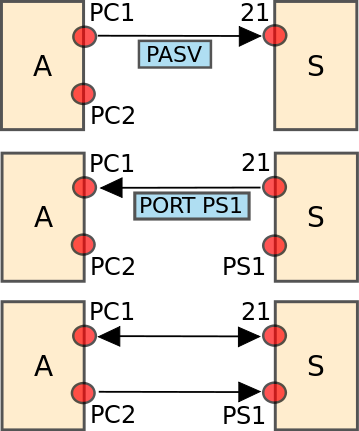
\includegraphics[width=0.5\textwidth]{FTPConnectionBuildup.png}\\
        \textit{A: Client -- S: Server\\}
    \end{center}
    
    Man unterscheidet zwischen Aktivem FTP und Passivem FTP:\\
    \textbf{Aktives FTP} wird vom Clienten mithilfe von PORT und EPRT initiiert und man unterscheidet wie oben beschrieben den Befehlskanal und den Datenkanal.\\
\textbf{Passives FTP} wird via PASV und EPSV Befehlen gestartet. 
Dieser Modus wird genutzt, wenn keine direkte Verbindung zum Clienten aufgebaut werden kann, etwas aufgrund einer Firewall oder Adressumschreibungen via NAT.
    
    \subsection{SMTP}
    \label{protocols:smtp}
    Das Simple Mail Transfer Protocol dient dem Austausch von Emails, 
    primär jedoch zum Senden und Weiterleiten 
    -- Zum Empfangen dieser dient üblicherweise POP3 oder IMAP.
    SMTP-Server liegen üblicherweise auf \textbf{Port 25} oder \textbf{587} für authentifizierte Mails.
    
    Normalerweise wird SMTP vom Mail User Agent ausgeführt, welcher sich zum SMTP-Server verbindet und dann dem Nutzer die Mails weiterleitet:
    
    \begin{center}
        \begin{tabular}{c|c|c}
            Client              &   Server          &                                   \\\hline
            telnet x.y.z 25     &                   & Der User Agent ruft auf           \\
                                &   220 Ready       & Server Meldet sich                \\
            EHLO Oi             &                   & Client identifiziert sich         \\
                                &   250 OK          & Server bestätigt                  \\
            MAIL FROM: <@.org>  &                   & Client definiert Absenderadresse  \\
                                &   250 OK          & Server bestätigt                  \\
            RCPT TO: <@.org>    &                   & Client definiert Empfängeradresse \\  
                                &   250 OK          & Server bestätigt                  \\
            DATA                &                   & Client initiiert die Email selbst \\
                            &   354 Start Input &                                   \\
            (MailInput)         &                   & Die Email wird geschrieben. Ein '.' beendet die Email.  \\
                                &   250 OK          & Server bestätigt die EMail.       \\ 
            QUIT                &                   & Client initiiert Verbindungsabbau \\
                                &   221 Closing     & Verbindung ist terminiert.    \\
        \end{tabular}
    \end{center}
    
    \subsection{Post Office Protokol (POP3)}
    \label{protocols:pop3}
    Das Post Office Protokol 3 dient dem Empfangen von Daten auf dem lokalen Gerät.
    Es ist das minimalste Protokol, da es lediglich Auflisten, Abholen und Löschen implementiert. 
    Im Gegensatz zu IMAP werden bei einem Pull-Request die Daten direkt vom Server gezogen, 
    wo diese auch gelöscht werden. Zudem ist keine permanente Verbindung zum Server notwendig. 
    Allerdings gibt es zwischen unterschiedlichen Mailclients keine einheitliche Synchronisierung -- Wird eine Mail gelesen, so können andere Klienten diese Information nicht erhalten.

    Um bei POP3 Datensicherheit zu gewährleisten wird APOP implementiert und/oder mittels SSL/TLS verschlüsselt. 

    Encryptete Kommunikation via POP3 wird entweder nach der Protocol Initiierung (durch Verwenden des STLS Kommandos) angefordert, 
    oder mit \textbf{POP3S}, welches sich zum Server mit \textbf{Transport Layer Security (TLS)} oder \textbf{Secure Sockets Layer (SSL)} am TCP Port 995 verbindet.
    
    \textbf{Befehle}: USER, PASS, STAT, LIST, RETR, DELE, NOOP, RSET, QUIT.

    \subsection{Internet Message Access Protocol (IMAP)}
    \label{protocols:imap}
    Bei dem Internet Message Access Protocol handelt es sich um ein Internet Standard Protocol, 
    dass von E-Mail Clients verwendet wird, 
    um E-Mail Nachrichten von einem Mail Server über eine TCP/IP Verbindung zu erhalten.

    Es erweitert POP3 um Userdefinierte Konfigurationen des Mailservers. 
    Bei einem Serverzugriff werden Kopien der Mails dem Server entnommen, 
    um Datenverlust vorzubeugen.
    Daher werden im Gegensatz zur POP3 Standard Konfigurationen E-Mails am Server gelassen,
    außer der User löscht diese explizit.

    Mittels einer \textbf{SSL Verbindung} kann über IMAPS eine sichere Verbindung erstellt werden.

    \paragraph{Der Datentransfer verläuft wie folgt:}
    \begin{verbatim}
    -- Der Server begrüßt den Clienten.
    -- Der Client authentifiziert sich.
    -- Der Server bestätigt.
    -- Der Client gibt einen Befehl ein (z.B. 'select Inbox').
    -- Der Server gibt Daten über vorhandene und gelesene Mails wieder.
    -- Der Client pullt die Mails oder Informationen.
    -- Der Server beantwortet je nach Befehl mit angefordertem Datensatz.
    -- ... Der Client meldet sich ab.
    -- Server terminiert die Verbindung.
    \end{verbatim}
    
    \subsection{Simple Network Management Protocol (SNMP)}
    \label{protocols:snmp}
    Das Simple Network Management Protocol dient der zentralen Überwachung und Steuerung von Geräten innerhalb eines Netzwerkes, als auch Fehlererkennung und -benachrichtigung. Es gilt daher als Protokol der Anwendungsschicht.
    
    \paragraph{SNMP Agents empfangen an den jeweiligen Geräten die Befehle:} 
    \begin{itemize}
        \item GET-REQUEST,
        \item GETNEXT-REQUEST,
        \item GETBULK,
        \item SET-REQUEST,
        \item GET-RESPONSE,
        \item INFORM-REQUEST,
        \item Trap.
    \end{itemize}
    Die 3 Get-Befehlspakete können vom Manager zu einem Agenten gesendet werden, um Daten anzufordern. Die Antwort erfolgt mittels Response-Paket.
    Mittels SET können Agenten konfiguriert werden.
    
    Sicherheitsprobleme: SNMP unterstützt keine Anmeldung mit Kennwort und Usernamen -- Es werden lediglich Communities zum Management verwendet, etwa PUBLIC (read-only) und PRIVATE(read-write).
    
    \subsection{Domain Name Service (DNS)}
    \label{protocols:dns}
    Der Domain Name Service bietet in Netzwerken die Namensauflösung der IPs und ist Teil des Application Layers -- Nicht zu verwechseln mit ARP/RARP im Link Layer.
    Ähnlich einem Telefonbuch wird bei einer Anfrage ermittelt wo die angeforderte IP liegt und übermittelt.

    Während DNS dezentral aufgebaut ist, gelten hierarchische Strukturierungen, in Form eines Baumes:
    \begin{center}
        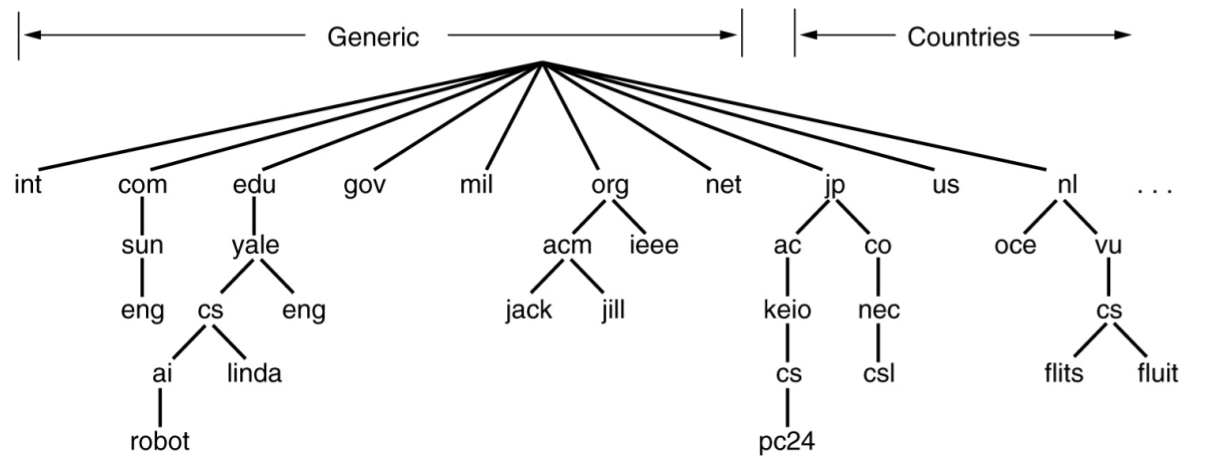
\includegraphics[width=\textwidth]{DNSNameSpace.png}\\
        \textit{Man iteriert von oben nach unten}.
    \end{center}
    Eine komplette Domain besteht aus der Konkatinierung aller Labels eines spezifischen Pfades. 
    Die Adresse 'de.sharelatex.com' wäre beispielsweise:
    \begin{verbatim}
         .
         |
        com
           \
            \
         sharelatex
             |
            de
    \end{verbatim}
    Jedes einzelne Label sind jeweils mindestes 1 Byte und maximal 63 Byte lang und enden mit einerm '.'.
    
    Die Adressauflösung geschieht anhand der Zusammenarbeit mehrerer DNS-Server.
    
    \begin{center}
        \begin{tabular}{l|l}
            Iterative & Recursive  \\\hline
        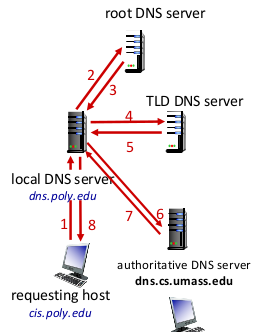
\includegraphics[width=0.4\textwidth]{DNSIterativeQuery.png} & 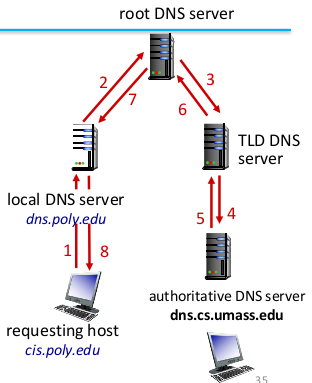
\includegraphics[width=0.4\textwidth]{DNSRecursiveQuery.png}   \\\hline\vspace{1em}
        \begin{minipage}{0.4\textwidth}
        Der Kontaktierte darüberliegende Server beantwortet mit der gesuchten IP oder mit einem weiteren DNSServer, welcher womöglich die Adresse kennt.
        \end{minipage}
        &
        \begin{minipage}{0.4\textwidth}
        Der Server fragt alle darunterliegenden Stationen nach der IP. Gibt es keine Nachricht, so wird die Anfrage dem darüberliegenden DNSServer weitergeleitet.\\
        \end{minipage}
        \end{tabular}
    \end{center}
    
    Für gewöhnlich werden Einträge von IPs in den jeweiligen Zonen unterscheidet.

    \pagebreak
    \subsection{Transmission Control Protocol (TCP)}
    \label{protocols:tcp}
    Das Transmission Control Protokol arbeitet auf der Transportschicht und dient der Datenübertragung. 
    TCP implementiert den sog. 'Handshake', 
    wobei ein sicherer Datenübertragungkanal zwischen Server und Client aufgebaut wird. 
    
    Dabei bietet TCP eine verlässliche,
    geordnete und auf Fehler überprüfte Übertragung eines Streams von \emph{Octets (Byte)} zwischen Applikationen
    von Host Systemen, die via einen IP Netzwerk miteinander kommunizieren.
    Es gilt als Stop-and-wait Protokol.
    
    \paragraph{Struktur des TCP-Segmentes:}
   
    \begin{verbatim}
    0                   1                   2                   3
    0 1 2 3 4 5 6 7 8 9 0 1 2 3 4 5 6 7 8 9 0 1 2 3 4 5 6 7 8 9 0 1
    +-+-+-+-+-+-+-+-+-+-+-+-+-+-+-+-+-+-+-+-+-+-+-+-+-+-+-+-+-+-+-+-+
    |          Source Port          |       Destination Port        |
    +-+-+-+-+-+-+-+-+-+-+-+-+-+-+-+-+-+-+-+-+-+-+-+-+-+-+-+-+-+-+-+-+
    |                        Sequence Number                        |
    +-+-+-+-+-+-+-+-+-+-+-+-+-+-+-+-+-+-+-+-+-+-+-+-+-+-+-+-+-+-+-+-+
    |                    Acknowledgment Number                      |
    +-+-+-+-+-+-+-+-+-+-+-+-+-+-+-+-+-+-+-+-+-+-+-+-+-+-+-+-+-+-+-+-+
    |  Data |           |U|A|P|R|S|F|                               |
    | Offset| Reserved  |R|C|S|S|Y|I|            Window             |
    |       |           |G|K|H|T|N|N|                               |
    +-+-+-+-+-+-+-+-+-+-+-+-+-+-+-+-+-+-+-+-+-+-+-+-+-+-+-+-+-+-+-+-+
    |           Checksum            |         Urgent Pointer        |
    +-+-+-+-+-+-+-+-+-+-+-+-+-+-+-+-+-+-+-+-+-+-+-+-+-+-+-+-+-+-+-+-+
    |                    Options                    |    Padding    |
    +-+-+-+-+-+-+-+-+-+-+-+-+-+-+-+-+-+-+-+-+-+-+-+-+-+-+-+-+-+-+-+-+
    |                             data                              |
    +-+-+-+-+-+-+-+-+-+-+-+-+-+-+-+-+-+-+-+-+-+-+-+-+-+-+-+-+-+-+-+-+        
    \end{verbatim}
    
    \paragraph{Merkmale:}
    \begin{description}
        \item [Full Duplex Data] Bi-directional data flow in same connection.\\MSS: maximum segment size.
        
        \item [Connection-oriented] Initializes Channel before sending and terminates channel once everything's been sent.
        \\Handshakeing (exchange of control messages).
        
        \item [Flow Control] Receiver controls sending rate of the Sender -- Empfänger übermittelt Überlauf des Empfangsbuffers.
        \item [Congestion Control] Bei zuvielen Daten von zuvielen Quellen: Verwurf von Daten auf der Netzwerkschicht durch Bufferoverflow.
        \item [Point-to-point] One sender, one receiver.
        \item [Reliable, in-order byte stream] No message boundaries.
        \item [Pipelined] TCP congestion and flow control set window size.
        
        \begin{center}
            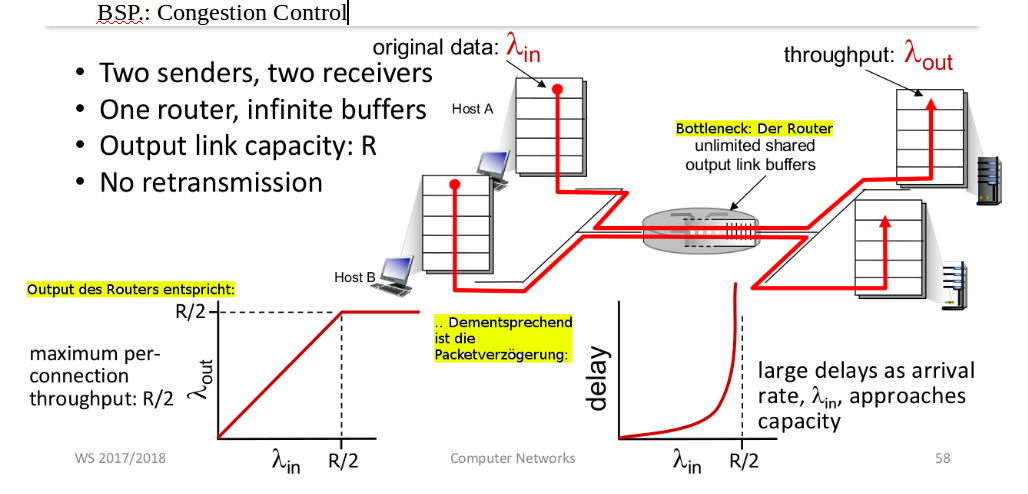
\includegraphics[width=\textwidth]{CongestionControl.png}
    \end{center}
    \end{description}

    \paragraph{Flow Control:}
    \label{protocols:TCP_flow_control}
    \begin{itemize}
        \item Der Empfänger zeig dem Sender das noch freier Buffer zur Verfügung steht, 
        indem ein \texttt{rwnd} Wert im TCP Header mitgesendet wird.
        \begin{itemize}
            \item \texttt{RcvBuffer} Größe wird mittels einer Socket Option gesetzt (Defaultwert typischerweise 4096 bytes).
            \item Viele OS setzen \texttt{RcvBuffer} automatisch.
        \end{itemize}
    \end{itemize}


    \paragraph{Congestion Control:}
    \label{protocols:TCP_congestion_control}
    \begin{itemize}
        \item Informally: "too many sources sending too much data too fast for network to handle."
        \item Different from flow control!
        \item Manifestations:
        \begin{itemize}
            \item Lost packets (buffer overflow at routers).
            \item Long delays (queueing in router buffers).
        \end{itemize}
        \item A top-10 problem!
    \end{itemize}
    
    \paragraph{Wichtige Flags bei TCP:}
    
    \begin{description}
        \item [SYN-Flag] Initiiere Channel,
        \item [FIN-Flag] Terminiere Channel,
        \item [ACK-Flag] Authentifiziert die ACK.
    \end{description}
    
    TCP im großem Ausmaß wird üblicherweise via Go-Back-N oder Selective Repeat implementiert.
    
    \paragraph{G-Back-N (GBN)}
    \begin{figure}[h!]
        \centering
        \caption{G-Back-N}
        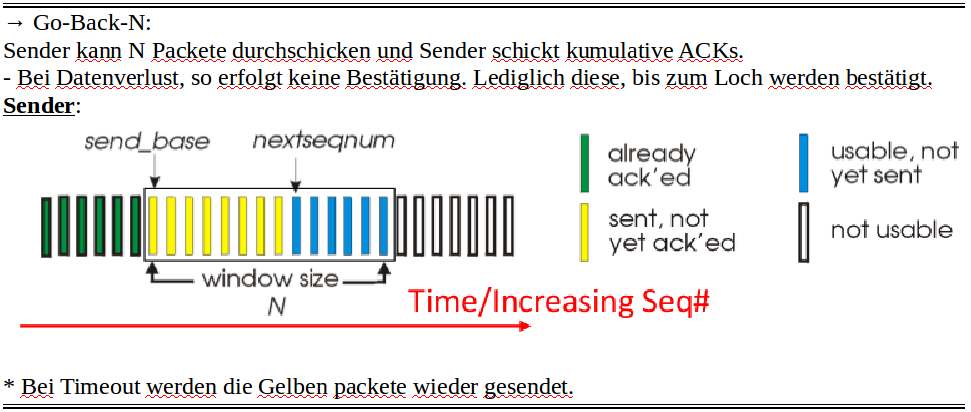
\includegraphics[width=0.8\textwidth]{GoBackN.png}
    \end{figure}

    \begin{itemize}
        \item Der Sender kann bis zu $N$ \textbf{unack'ed Pakete} in der Pipeline haben.
        \item Der Empfänger sendet nur ein kumulatives \textbf{ack} 
        \begin{itemize}
            \item Wenn eine Lücke darin ist, wird kein \textbf{ack packet} gesendet.
        \end{itemize}
        \item Sender hat einen Timer für das älteste \emph{unack} Paket.
        \begin{itemize}
            \item Wenn der Timer ausläuft, werden alle \emph{unack} Pakete wiedergesendet.
        \end{itemize}
    \end{itemize}
    
    
    \paragraph{Selective Repeat}
    \begin{figure}[h!]
        \centering
        \caption{Selective Repeat}
        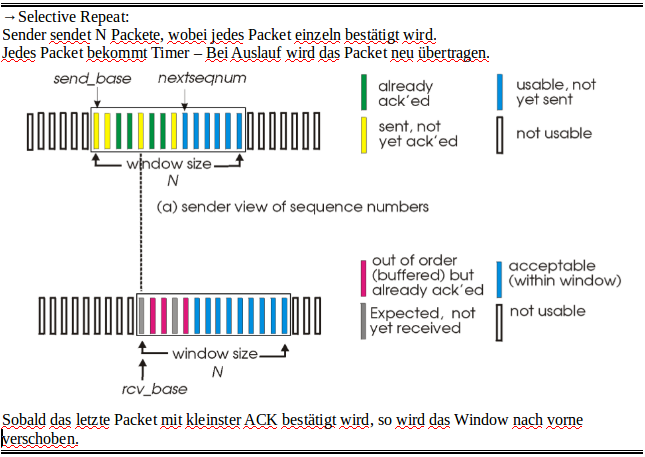
\includegraphics[width=0.8\textwidth]{SelectiveRepeat.png}
    \end{figure}
  
    \begin{itemize}
        \item Der Empfänger sendet individuelle acknowlegdes für jedes korrekt erhaltene Paket. 
        \begin{itemize}
            \item Buffered die Pakete, falls notwendig, für eventuelle \emph{in-order delivery} an den upper layer.
        \end{itemize}
        \item Der Sender muss nur die Pakete wieder senden, für welche das ACK noch nicht erhalten wurde.
        \begin{itemize}
            \item Daher ein Sender Timer für jedes unACK'ed Paket.
        \end{itemize}
        
    \end{itemize}

    \subsection{UDP}
    \label{protocols:udp}
    UDP ist im Grunde das Gegenstück zu TCP: Verbindungsfreie Datenübertragung ohne Sicherheiten, Zustandslose, jedoch weitaus schneller als TCP, aufgrund des fehlenden Overheads durch den Handshake und mit kleinerem Header.
    
    \paragraph{UDP-Struktur:}
    
    \begin{verbatim}
        0       7 8     15 16    23 24    31  
        +--------+--------+--------+--------+ 
        |     Source      |   Destination   | 
        |      Port       |      Port       | 
        +--------+--------+--------+--------+ 
        |                 |                 | 
        |     Length      |    Checksum     | 
        +--------+--------+--------+--------+ 
        |                                     
        |              Payload 
        |           e.g. AppData
        +---------------- ...                 
    \end{verbatim}
    $\rightarrow$ Daraus resultiert: Das kleinste UDP-Segment ist 8 Byte lang - Mit leerem Payload und den Headern zu je 2 Byte.
    
    
    \subsection{BGP}
    Das Border Gateway Protocol ist das Routingprotokoll das Autonome Systeme miteinander verbindet. Es ist Teil der Anwendungsschicht und basiert auf TCP.
    
    Im Rahmen von BGP existieren \textbf{eBGP}, external BGP und \textbf{iBGP}, internal BGP. Internal BGP steht für das Routing innerhalb eines Subsystemes und External BGP steht für das Routing von Paketen in andere BGP-Systeme.
    
    Das iBGP trackt hierbei stets, welche Elemente im jeweiligen System sind. Wird eine Komponente hinzugefügt, so wird dies über den eBGP-Knoten weitervermittelt.
    
    \begin{center}
        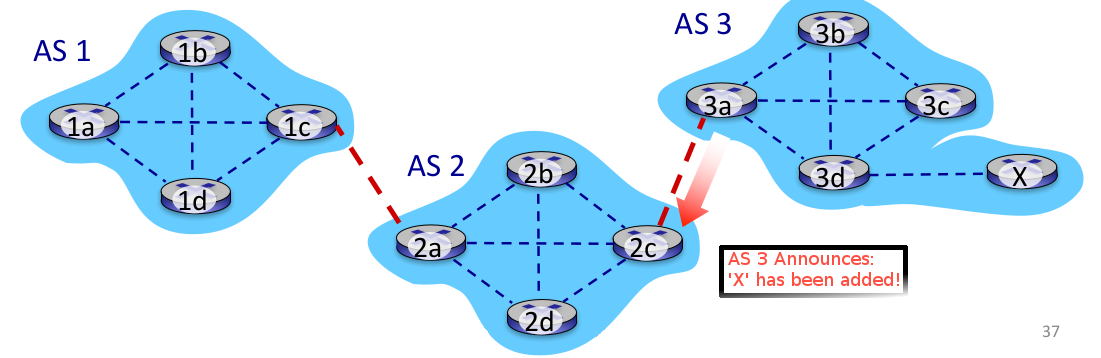
\includegraphics[width=\textwidth]{BGP.png}
        \textit{AS2 informs AS1 aswell that AS3 has added 'X'}
    \end{center}
    
    Das Routing innerhalb von BGP basiert auf mehreren Möglichkeiten:
    \begin{enumerate}
        \item Lokale Preferenz
        \item Shortest AS-Path
        \item Closest NEXT-HOP -- Also known as Hot Potatoe Routing
        \item Other, specifiable Criteria or identifiers.
    \end{enumerate}
    
    
    \subsection{OSPF}
    Das Open Shortest Path First ist ein Link State-Protocol und basiert auf dem Dijkstra-Algorithmus. Es ist im Gegensatz zu BGP in der Vermittlungsschicht angesiedelt.
    
    Der Dijkstra-Algorithmus:
    \begin{center}
        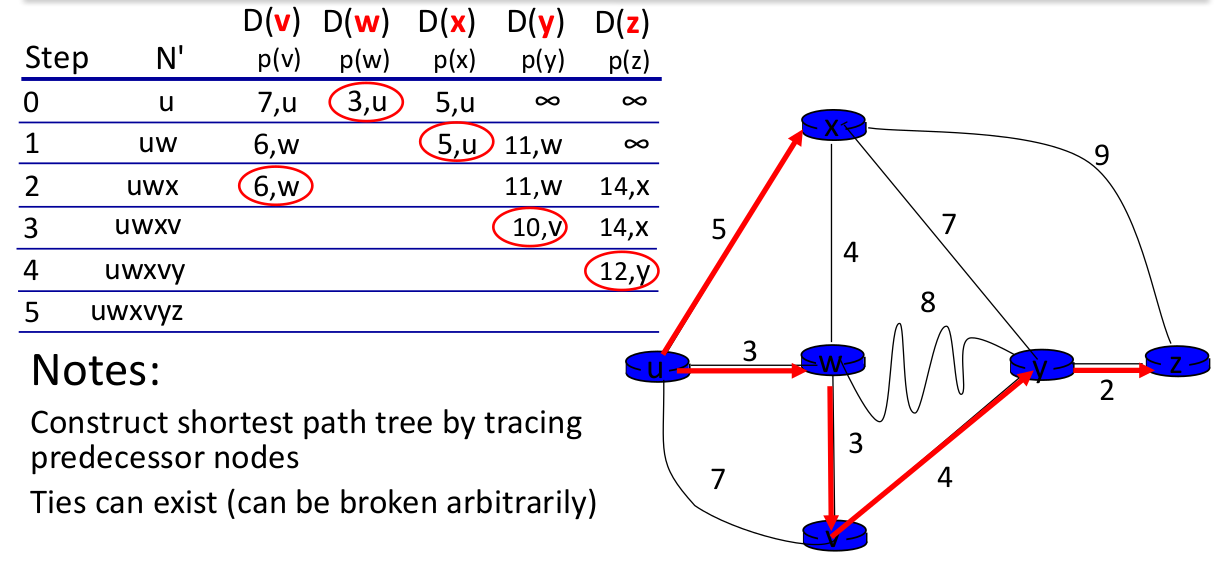
\includegraphics[width=\textwidth]{Dijkstra.png}\\
        \textit{Wähle günstigste Kante für jeden Fall. Beachte noch offene Knoten!}
    \end{center}
    
Alternativ ist auch der Distanz-Vektor Algorithmus anwendbar:
    \begin{center}
        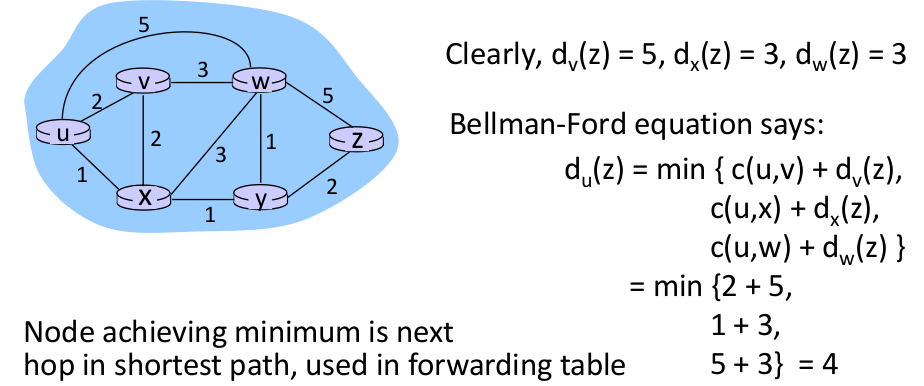
\includegraphics[width=\textwidth]{DistanceVector.png}\\
    \textit{Wähle Minimum aller Pfade von Knoten a zu b, wobei $d_u$ die Distanz zum Knoten u von Knoten $d(z)$ darstellt.}
    \end{center}
    
    Es garantiert schleifenfreies Routing, es überwacht Nachbarn (Area-Konzept) und ist damit leichter zu warten, es unterstützt Klassenlose Internetadressierungen und kann im Fehlerfall des Routings das Bidirectional Forwarding Detection-Protokoll nutzen.
    
    OSPF hält sich beim Routing immer an eine spezifische Hierarchie:
    \begin{center}
        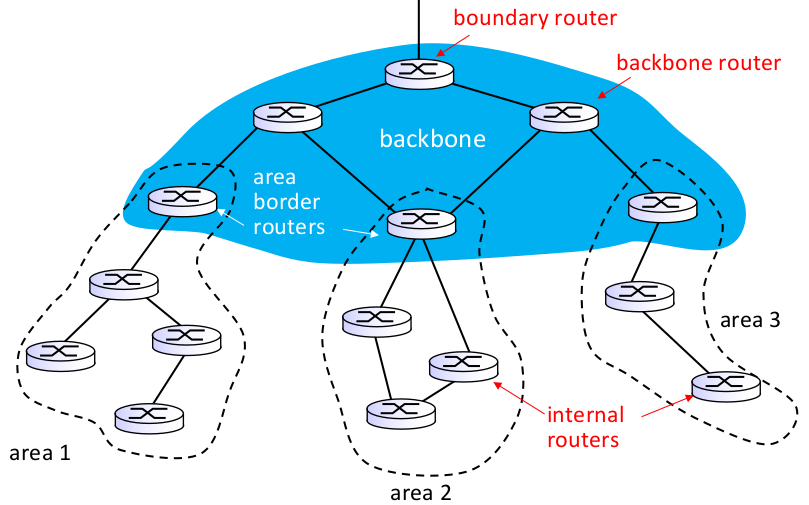
\includegraphics[width=\textwidth]{HierarchicalOSPF.png}
    \end{center}
    
    \subsection{SDN}
    Das Software-Defined Networking ist ein, umgangssprachlich genannter, Clusterfuck mehrerer Protokolle, die aufeinander aufbauen und via Hardware gemanaged werden.
    Es implementiert Flow-Based forwarding, es trennt Dataplane und Control Plane mittels Switches und verfügt über ein programmierbares Netzwerk.

    Prinzipiel gibt es die SDN Control Applications, den SDN Controller und die SDN-Controlled switches.
    \begin{center}
    \begin{tabular}{c|c}
        \begin{minipage}{0.6\textwidth}
        \begin{enumerate}
            \item Die Kontrolapplikationen dienen dem konkreten Steuern des SDN.
            \item Der SDN Controller erhält die Konsistenz des Netzwerkes. Als Verteiltes System hat es Zugriff auf sowohl Applikationen als auch Switches.
            \item Die SDN Switches dienen dem Forwarding.
        \end{enumerate}
        \end{minipage}
        &
        \begin{minipage}{0.3\textwidth}
        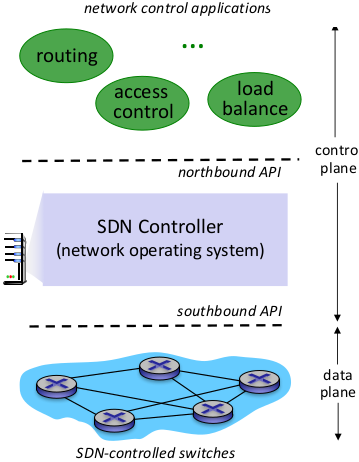
\includegraphics[width=\textwidth]{SDNComponents.png}   \\
        \end{minipage}
    \end{tabular}
    \end{center}

    \subsection{TDMA, FDMA, CDMA}
    TDMA, FDMA und CDMA dienen beispielgebend dazu, wie man Verbindungen effektiv einteilen kann.
    \begin{enumerate}
        \item TDMA\\
        Im Time Division Multiple Access-Verfahren bekommt jeder User mittels zeitlichem Multiplexing einen Zeitrahmen zugesprochen, in welchem er Senden darf. Hierfür bekommt dieser User den gesamten Frequenzbereich zugesprochen.
        \item FDMA\\
        In Frequency Division Multiple Access bekommt jeder User eine fixierte Frequenz auf welcher er senden darf.
        \item CDMA\\
        Code Division Multiple Access gilt dem Wireless Bereich. Man kann simultan senden, wobei encodieren der Daten den Sender und Empfänger spezifizieren.
    \end{enumerate}
    \begin{center}
        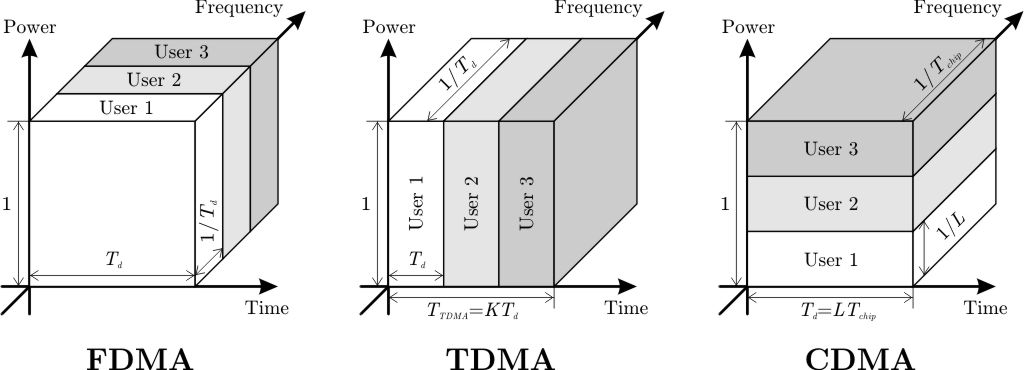
\includegraphics[width=\textwidth]{TDMACDMAFDMA.jpg}
    \end{center}
    
    \subsection{SALOHA}
    SALOHA, oder Slotted Additive Links On-Line Hawaii Area bedient sich dem TDMA, wobei jeder Slot Zeitslot miteinander synchronisiert wird.
    Sobald ein Frame zur Übertragung kommt, so wird dies unmittelbar für den nächsten Zeitslot eingetragen. Bei Kollissionen wird dem jeweiligen Paket ein Zeitstempel verpasst und diesem entsprechend in einen neuen Slot eingetragen.
    \begin{center}
        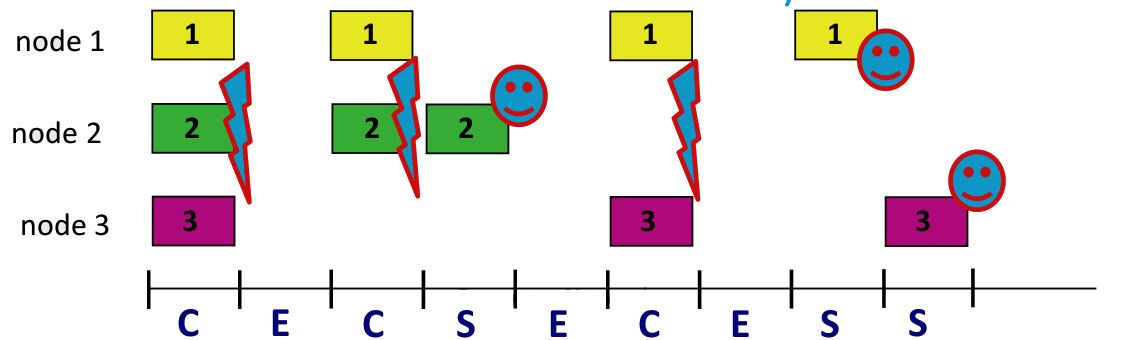
\includegraphics[width=\textwidth]{Aloha.png}
    \end{center}
    
    Eine weitere Version, das PURE oder unslotted ALOHA ist simpler, ohne Synchronisation. Hierbei werden eintreffende Frames sofortig gesendet.
    Bei einer Kollission werden die Übetragungen abgebrochen und man erwartet eine ACK des Empfängers -- Siehe CSMA/CD.
    
    \subsection{CSMA/CD}
    Das Carrier Sending Multiple Access/Collision Detection ist eine umfassende Übertragungsstruktur, aufbauend auf TDMA.
    In CSMA wird aktiv mitgehört wann eine Station etwas sendet. Wenn der Übertragungskanal unbenutzt ist, so startet unmittelbar die Übertragung. Ist der Kanal besetzt, so wird die Übertragung verlegt. Generell dient es im Ethernet.
    
    Einzelne Übertragungsstationen agieren in einem spezifischen Frequenzbereich:
    \begin{center}
        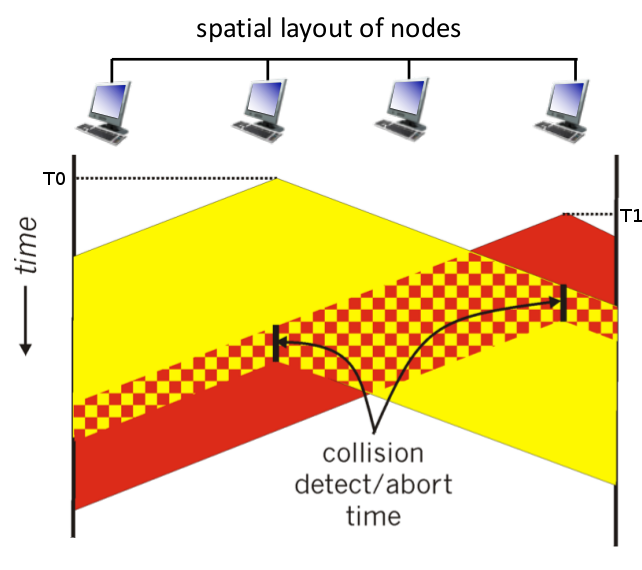
\includegraphics[width=\textwidth]{CSMACD.png}\\
        \textit{Kollision entdeckt -- erwarte ACK}
    \end{center}
    
    Wird keine Kollission entdeckt, so wird die Datei normal übertragen. Sollte eine Kollision entdeckt werden, so wird die Übertragung abgebrochen. Und die Übertragung wird später ausgeführt, wobei man per Kollission exponentiell lange wartet.
    
    \subsection{CSMA/CA}
    Carrier Sensing Multiple Access/Collision Avoidance unterscheidet sich weitgehend von dessen Konterpart, CD.
    Es kombiniert mehrere Token-Topologien zu einem Protokoll und wird üblicherweise für 802.11, also WLAN, genutzt.
    
    Innerhalb eines Netzwerkes bekommt der Router Anfragen, 'Requests to send', von den jeweiligen Geräten. Der Server sendet anschließend an alle Beteiligten im Netzwerk, dass der spezifisch gewählte Knoten senden wird und damit der Kanal besetzt ist. Nach der Datenübertragung sendet der Server eine ACK an alle, um den freien Kanal anzukündigen.
    \begin{center}
        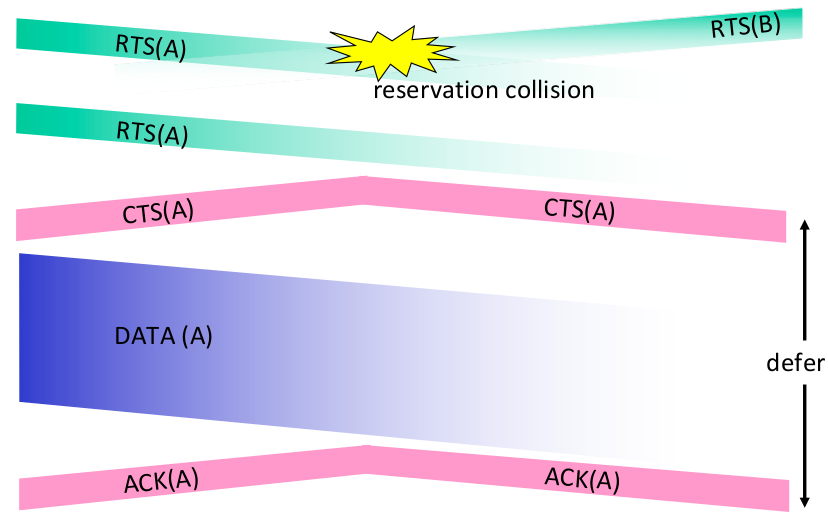
\includegraphics[width=\textwidth]{CSMACA.png}
    \end{center}

    \subsection{ARP}
    Das Address Resolution Protocol ist Teil der Netzzugangsschicht und dient der Zuordnung einer IPv4 Adressierung in Ethernet-Netzen zu einer MAC-Adresse. (IPv6 -- Neighbor Discovery Protocol)
    Die Adresse einer jeder Schnittstelle ist dabei, theoretisch gesehen, weltweit eindeutig. Wird die MAC-Adresse des Zielrechners nicht spezifiziert, so ist ein IP-Paket unzustellbar. Jedoch kann man mithilfe von ARP die MAC-Adresse des Zielrechners.
    
    \subsection{IEEE 802.11 Wireless LAN}
    Das Wireless Local Area Network ist eine Verbindung via Funk. Man spezifiziert hier wiederum zwischen verschiedenen Frequenzbereichen, wodurch die Kompatibilität zu anderen Versionen nicht gegeben sein muss.
    



% TODO :: Implement programs. Use verbatim for code plx -- If at all
\section{Networking in Java}
    \subsection{Processes}
    \subsection{Threads}
    \subsection{Readers and Writers}
    \subsection{Sockets and Exceptions}
% Do this? \subsection{Bounded Buffer}
   
\section{Begriffe und Definitionen}
    \begin{enumerate}[$\bullet$]
        \item \textbf{Das Internet}:
        Das Internet ist ein weltweiter Verbund von Rechnernetzwerken und autonomen Systemen (AS). Datenaustausch zweier Systeme wird spezifiziert in Protokollen, beschrieben in RFCs der Internet Engineering Task Force (IETF).\\
        \textit{Vorläufer}: ARPANet -- Advanced Research Project Agency, US-Militär gefolgt von TCP/IP, DNS, Usenet und darauf Kommerz-WWW: 1991 weltweit öffentlich verfügbar.
        \item \textbf{Netzwerktopologie}
        Eine Netzwerk-Topologie ist die physikalische Anordnung von Netzwerk-Stationen, die miteinander verbunden sind. Sie ist unterteilbar in dessen \textit{Logik -- Wo befindet sich ein Gerät im Netzwerk \& Physik -- Ports und Kabel }. 
        Typische Topologien sind:
% TODO: Align this tabular accordingly.        
        \begin{center}
            \begin{tabular}{c|c}
            Bus/Kette & Ring  \\
            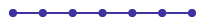
\includegraphics[]{Topologie_Chain.png}     &  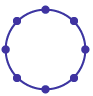
\includegraphics[]{Topologie_Ring.png} \\\hline
            Stern     &  Baum \\
            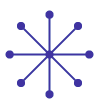
\includegraphics[]{Topologie_Star.png} & 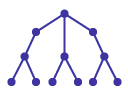
\includegraphics[]{Topologie_Tree.png}       \\\hline
            Mesh & Fabric   \\
            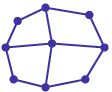
\includegraphics[]{Topologie_Mesh.png} & 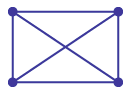
\includegraphics[]{Topologie_Fabric.png}       \\
            \end{tabular}
        \end{center}
        \item \textbf{Servicetypen}:\\ $\bullet$ Connection oriented Services, auch 'Verbindungsorientierte': Ähnlich TCP. Vergleichbar mit einem Telefonanruf, beispielsweise Reliable Data Streams (Sequence of Pages or Remote Logins).\\
        $\bullet$ Connectionless Services, auch 'Verbindungslose': Ähnlich UDP. Vergleichbar mit Briefpost, oft in Form von Emails und Database querys.
        \item \textbf{Circuit Switching und Packet Switching}:\\ $\bullet$ Bei Circuit Switching werden Leitungen gänzlich reserviert. Solange 2 Medien miteinder kommunizieren, können andere u.U. nichts versenden da die Leitung blockiert ist (no Sharing). Implementiert via FDMA (4 User auf 4) oder TDMA (4 User auf 1 Kanal).\\
        $\bullet$ Packet Switching bedient sich dem Aufteilen der Daten in Pakete. Zieladresse gibt an wohin das Paket gesendet werden muss, wobei die Routen je nach Forwarding-Funktion variieren.

    \begin{center}
% TODO: Format this
        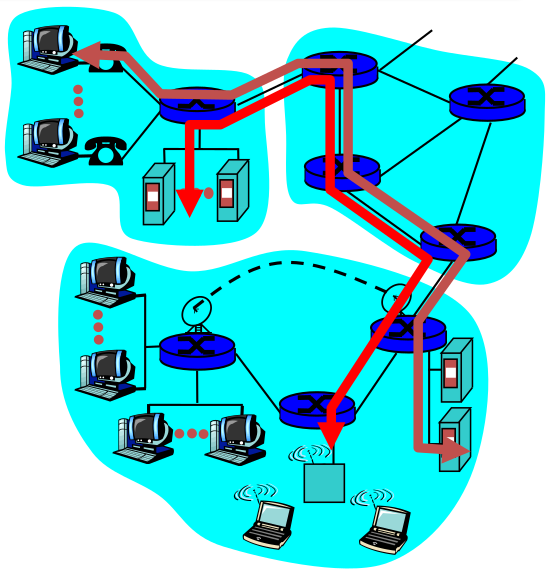
\includegraphics[width=0.4\textwidth]{CircuitSwitching.png}\\
        \textit{Circuit Switching within a network.}\\
        
        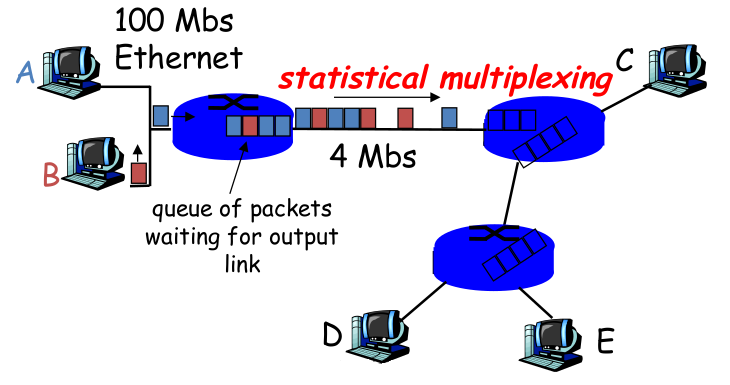
\includegraphics[width=0.7\textwidth]{PacketSwitchingStatistical.png}\\
        \textit{Statistical Packet Switching.}\\
        
        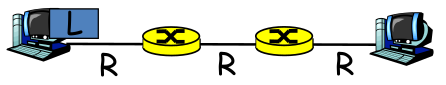
\includegraphics[width=0.8\textwidth]{PacketSwitchingSF.png}\\
        \textit{Store And Forward Switching.}\\
    \end{center}
                
% TO CONTINUE 
        \item Netzwerktypen:
        \begin{enumerate}
            \item Digital Subscriber Line\\
            Nutzt Telefonverbindung zur Verbindung zum Netzwerk, DSLAM.  
            \item Cable Network\\
            FDMA: Mehrere Nutzer hängen an einem Kabel.
            \item Home Network\\
            Typisches Heimnetzwerk mit zum Route verbundene Geräte.
            \item Ethernet oder Enterprise Access Networks\\
            Geräte sind zu einem Switch verbunden, welche mit ISP gekoppelt sind. 
        \end{enumerate}
        \item Multiplexing/Demultiplexing\\
        Beschreibt das Hinzufügen/Entfernen von Steuer- und Kontrolinformationen.
        \item Congestion Control und Flow Control\\
        $\bullet$ Congestion Control: Aufgrund zuvieler Quellen und Sender -- Datenverwurf auf 2ter Schicht.
        $\bullet$ Flow Control: Empfänger benachrichtig Sender Datenüberlauf im Routerbuffer.
        Flow Control:
        \item Reliable Data Transfer\\
        Zuverlässiger Datentransfer wird üblicherweise mittels verschiedener States gewährleistet. Vgl.: TCP
        \item Forwarding and Routing\\
        $\bullet$ Forwarding beschreibt den zu wählenden Pfad des Paketes.\\
        $\bullet$ Routing beschreibt den Pfad, welches das Paket zurückgelegt hat.\\
        \item MAC Addressen \\
        Media Access Control-Adressen konkretisieren das Gerät innerhalb eines Netzes -- Teil der 2. Schicht.
        Es gibt mehrere Arten der Syntax: 00-80-41-ae-fd-7e, wobei die Zeichentrennung via ',' '.' gesetz wird. Selten gibt es auch keine Zeichentrennung und es ist eine Zeichenkette.
        \item IPv4 und IPv6
% TODO
        \item Routing Algorithm Classifications
        Es gibt mehrere Arten von Routing Algorithmen.
        \item Autonomous Systems in Scalable Routing
        \item Hot Potato Routing
        \item IP-Anycast
        \item Multiple Access Protocols
        \item Channel Partitioning
        \item The 5G Atom
    \end{enumerate}
    \subsection{ Weitere Übertragungstypen }
    \begin{enumerate}
        \item Adaptive Streaming 
        \item Client-Server Communication
        \item Request-Response Protokol
        \item Stop-and-Wait
        \item Go-Back-N
        \item Selective Repeat
        \item Classless Interdomain Routing \& Network Address Translation % Put this elsewhere?
        \item Multicast 
        \item OpenFlow
        \item Network Management
        \item Ethernet, Switches \& Routers
        \item Flooding % Probably add this to ethernet & Switches
        \item The Wireless Network
        \item IEEE
        \begin{enumerate}
            \item 802.2 Logical Link Protocol - Medienzuteilung bei MAC
            \item 802.4 Token Bus
            \item 802.5 Token Ring
            \item 802.11 WLAN
        \end{enumerate}
    \end{enumerate}
    
    \subsection{Berechnungen}
    \subsubsection{Graph Abstractions of the Network}
    \begin{enumerate}
        \item Dijstra
        \begin{center}
            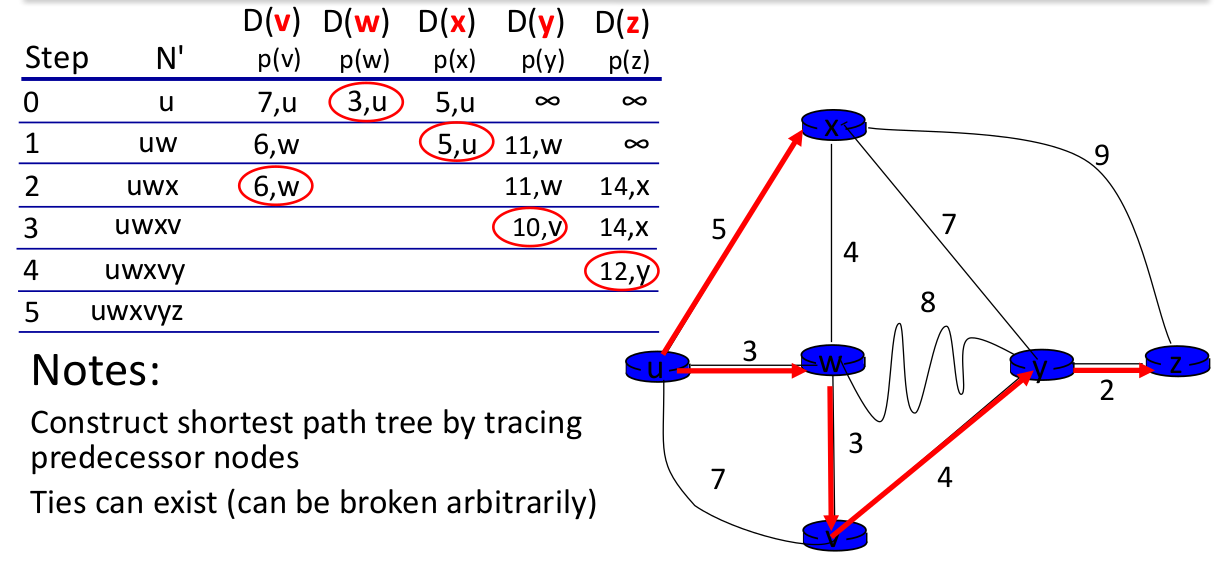
\includegraphics[width=\textwidth]{Dijkstra.png}\\
            \textit{Wähle günstigste Kante für jeden Fall. Beachte noch offene Knoten!}
        \end{center}
        \item Distance-Vector
        \begin{center}
            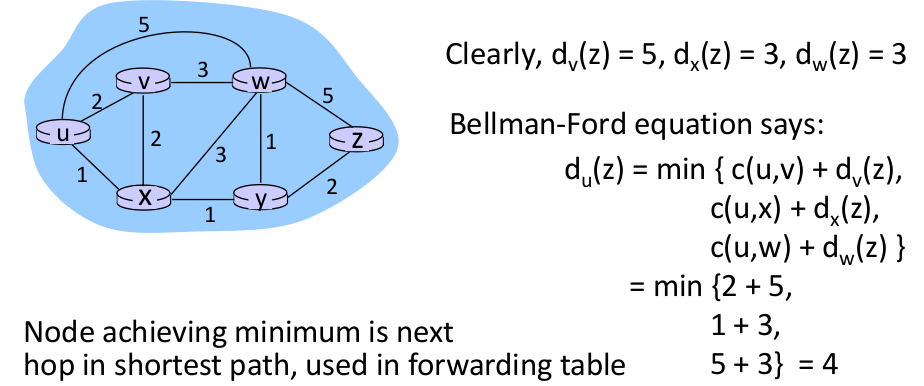
\includegraphics[width=\textwidth]{DistanceVector.png}\\
        \textit{Wähle Minimum aller Pfade von Knoten a zu b, wobei $d_u$ die Distanz zum Knoten u von Knoten $d(z)$ darstellt.}
        \end{center}
        
    \end{enumerate}
    \subsubsection{ IP-Addressberechnungen}
    IP-Adressberechnungen basieren auf deren Klassifizierung bzw. auf deren Netzanteil.
        IPv4 -- Adressberechnung
        Bei einem Subnetz von 11111111.11111111.11111111.00000000 (255.255.255.0) wird der Netzteil auf 192.168.0 festgelegt $\leftrightarrow$ E.g. wir besitzen 8 Bits für unsere Hostadressen.\\
        $\rightarrow$ Der Netzname ist predefiniert mit .0\\
        $\rightarrow$ Der Broadcsat liegt auf .255\\
        $\rightarrow$ Wir können damit noch $2^8 - 2$ Adressen belegen, dementsprechend hat dieses Netz noch 254 Adressen zur Verfügung.\\
        
        Dies funktioniert analog mit dem Klassenlosen IPv4 Verteilungsprinzip, bei welchem man die höchstwertigen Bits (von Links) dem Netzteil zuspricht. Der Rest resolviert die Anzahl an zu vergebene Adressen.\\
        Für einen Netzteil von 192.168.120 $\leftrightarrow$ 11000000.10101000.01111 existiert ein möglicher Host-Adressbereich von $32-8-8-5 = 11$ setzbaren Bits, dementsprechend haben wir $2^11 - 2 = 2046$  Adressen. \\
        
    IPv6 -- Adressberechnung\\
        .. verläuft nach demselben Schema wie bei IPv4. Die Adressen werden in ihre Bits transformiert und es werden Netz- und Hostadressbereiche eingeteilt.
        Der Wert nach einer IPv6 Adresse (.../12) beschreibt die Anzahl der Bits für den Netzanteil. Der Rest der Adresse beschreibt den Hostanteil. 
        
        IPv4 to IPv6
        Für eine IPv4, z.B. 192.168.99.1 erzeugt man die IPv6 Adresse durch Umschreibung in Hexadezimal.
        Wähle jedes Oktet und dividiere durch 16, um eine Hexadezimalzahl zu erzeugen.
        \begin{verbatim}
            192 -> C0       168 -> A8       99 -> 63        1 -> 01
        \end{verbatim} 
        Damit ist die IPv6-Representation von 192.168.99.1 die Konkatenation der Hexadezimalwerte C0A8:6301.
        Die Umsetzung ist vordefiniert nach dem Schema 2002:<32-Bit IPv4>:<16-Bit Network>::/64
        Die vollständige IPv6-Adresse lautet 2002:C0A8:6301::1/64.  (64 $\rightarrow$ '0' als 2ter Parameter von Links)
        
        IPv6 to IPv4
        Analog, nur rückwärts. Man extrahiert die 32-Bit aus der IPv6 Adresse und wandelt um.
        Mit C0A8 6301 haben wir insgesamt 8 Hexawerte zu je 4 Bit, dies entspricht 32 Bit. Wandle *16 in eine Dezimalzahl um und interpretiere das Ergebnis u.U. in Binärdarstellung.

    \subsubsection{ Link Layer - Parity Checking }
    \subsubsection{ Cyclic Redundancy Check}
    Die Zyklische Redundanzberechnung dient der Fehlerkorrektur in Datenpaketen. Zur Datenüberprüfung wird ein Berechnungsverfahren angewandt und wenn dessen Ergebnis 0 ist, so ist der Datenblock fehlerfrei. Es dient jedoch nur zur Erkennung zufälliger Fehler, nicht zur Bestätigung der Paket-Ganzheit.
    
    Es basiert auf der Polynomdivision und die Folge der zu übertragenden bits werden als binäres Polynom betrachtet: 1001 ist beispielsweise: $1*x^3 + 0*x^2 + 0*x^1 + 1*x^0$.
    Die Bitfolge wird durch ein festzulegendes Generatorpolynom mod 2 geteilt, wobei ein Rest bleibt. Dieser ist der CRC-Wert. Bei der Datenübertragung wird dieser Wert an den originalen Datenblock angehängt.
    
    Zur Verifikation wird der Datenblock mit angehängtem CRC-Wert als Binärfolge interpretiert und erneut durch das CRC-Polynom Modulo geteilt. Ist das Ergebnis 0, so gibt es keinen Fehler.
    
    
    Bsp.:
    CRC-Polynom: 110101
    Datenblock: 11011
    Der Datenblock mit Anhang ist nun 11011|00000, wobei die Anzahl der 0en der Länge des CRC-Polynoms -1 entspricht. Man erinnere sich: Das Exklusive-Or erzeugt Ergebnisse wie folgt:
    \begin{verbatim}
        0 ^ 0 = 0       1 ^ 1 = 0
        0 ^ 1 = 1       1 ^ 0 = 1
    \end{verbatim}
    Mittels Exklusive-OR wird nun der Block mit Anhang durchdividiert:

    \begin{verbatim}
    1101100000
    110101
    ----------
    0000110000
        110101
    ----------
         00101   -> Rest
    \end{verbatim}
    Der Rest, 00101 wird nun dem originalen Datenblock angehänt und komplett übertragen: 1101100101
    
    Bei Datentransfer wird erneut durch das CRC-Polynom dividiert:
    \begin{verbatim}
    1101100101
    110101
    ----------
    0000110101
        110101
    ----------
         00000
    \end{verbatim}
    Hierbei haben wir den Restwert 0 und es ist damit kein Fehler aufgetreten.
    
    \subsubsection{ CDMA Encoding/Decoding}
    
% Do not subsection the questions. It overkills the table of contents
% If questions found: Also add into Solutions.
% Lösungen in die section darunter.
\section{Typische Klausurfragen \& Fallbeispiele}
    \subsection{Probeklausur WS2016/2017, 3. Termin}
    \begin{enumerate}
        \item \textbf{ISO/OSI vs TCP-Referenzmodell}: Worin unterscheidet sich das ISO/OSI- vom TCP/IP Referenzmodell
        \item \textbf{Transport}: Beschreibe die allgemeinen Eigenschaften von TCP bzw. UDP.
        \item \textbf{HTTP}: Beschreibe HTTP (a) allgemein, hinsichtlich (b) persistenter Verbindungen, (c) Zustände und (d) Caches.
        \item \textbf{Transportschicht}: Beschreibe und Skizziere die TCP-Verbindungsaufbau und TCP-Verbindungsabbau.
        \item \textbf{Netzwerkschicht}:
        Nenne und beschreibe die drei Hauptfunktionen der Netzwerkschicht und nenne die zwei bekanntesten Routingalgorithmen.
        \item \textbf{Netzwerkschicht}: Beschreibe IPv4 bzw. IPv6 und gehe auf Unterschiede ein und skizziere mögliche Ansätze zum Übergang von IPv4 und IPv6.
        \item \textbf{Sicherungsschicht}: Beschreibe CSMA/CD und CSMA/CA. Wo werden die Methoden eingesetzt?
        \item \textbf{Sicherungsschicht}: Beschreibe ARP.
        \item \textbf{Rechnernetze Allgemein}: Beschreibe die Funktionsweise und Unterschiede von paketvermittelnden und leitungsgebundenen Netzwerken.
    \end{enumerate}

    \subsection{Frei erfundene Bsp.}
\subsubsection{Theorie}
    \begin{enumerate}
        \item Ordne folgende Protokolle den Schichten des TCP-Modelles zu:
        \begin{center}
            \begin{tabular}{l|lll|l}
                SMNP        & $\bullet$ & & $\bullet$ &  Anwendungsschicht   \\
                POP3        & $\bullet$ & & $\bullet$ &  Transportschicht    \\
                ARP         & $\bullet$ & & $\bullet$ &  Vermittlungsschicht \\
                DNS         & $\bullet$ & & $\bullet$ &  Netzzugangsschicht  \\
                TLS         & $\bullet$ & & $\bullet$ &                      \\
            \end{tabular}
        \end{center}
        \item Was ist der Unterschied zwischen Flow Control und Congestion Control?
        \begin{itemize}
            \item An allocation problem that occurs at every level is how to keep a fast sender from swamping a slow receiver with data.
            \item Feedback from the receiver to the sender is often used. This subject is called \textbf{flow control}.
            \item Sometimes the problem is that the network is oversubscribed because too many computers want to send too much traffic,
            and the network cannot deliver it all. This overloading of the network is called \textbf{congestion}.
        \end{itemize}
        \item Was sind die unterschiedlichen Elemente eines Wireless Networks und wie arbeiten sie miteinander?
        \item Was passiert wenn man innerhalb eines WLan-Netzwerkes den Standort wechselt? 
        \item Was sind die 5 Eckpfeiler des 5G Atoms und welche Teilbereiche gibt es?
        \item Was bedeutet ''Multiple Access'' im Rahmen des IEEE 802.11?
        \item Was sind nennenswerte Unterschiede zwischen ARP und DNS?
        \item Worin unterscheiden sich Router und Switches?
        \item Wie funktioniert der Link Layer und was ermöglicht dieser? Skizziere!
        \item Wie unterscheiden sich TDMA, FDMA, CDMA? Skizziere.
        \item Wie funktioniert BGP? Gibt es äquivalente Protokolle?
        \item Welche Arten der Datenübertragungen gibt es und welche grundlegenden Protokolle werden dafür implementiert? 
        \textit{Tip: Uni-Cast sendet von 1 zu 1 weiterem.}
        \item Wie funktioniert SDN?
        \begin{itemize}
            \item \textbf{Key Characteristics:}
            \begin{itemize}
                \item Flow-based forwarding,
                \item Separation of data plane and control plane,
                \item Network control functions: external to data plane switches,
                \item A programmable network.
            \end{itemize}
            
            \item \textbf{Network control applications:}
            \begin{itemize}
                \item Brains of control,
                \item Unbundled: e.g., by 3rd party distinct from routing vendor or SND controller.
            \end{itemize}

            \item \textbf{SDN controller:}
            \begin{itemize}
                \item Maintain network state information,
                \item Interacts wiht network control application above via northbound API,
                \item Interacts with network switches below via southbound API,
                \item Implemented as distributed system for perfomance, scalability, fault-tolerance, robustness.
            \end{itemize}

            \item \textbf{Implementations:}
            \begin{itemize}
                \item OpenFlow,
                \item OpenDaylight.
            \end{itemize}
        \end{itemize}
        \item Was sind Grundfunktionalitäten der Applikationsschicht. Welche Protokolle werden hier implementiert?
        \item Wie unterscheiden sich Data Plane und Control Plane? Gibt es unterschiedliche Variationen des Control Plane?
        \item Wie wird ein IPv6 Paket behandelt, sollte man lediglich IPv4 weitersenden können?
        \item Welche Versionen von HTTP existieren und was sind Unterschiede zwischen den einzelnen Versionstypen? Ist HTTP ein sicheres Protokoll?
    \end{enumerate}
    \subsubsection{Berechnungen}
    \begin{enumerate}
        \item I seriously fucking hope this wont come.
        \item Welche Arten der IP-Adressierungen gibt es? Wie werden Geräte adressiert? % Add bsp
    \end{enumerate}
    \subsubsection{Wahr oder Falsch}
    \begin{enumerate}
        \item IEEE 802.11 ist ein Transportprotokoll.
        \item Mithilfe der Datenrate-adaption kann man Datenqualität optimieren. Das SNR verstärkt diese Optimierung.
        \item DAS SNR ist eine relative Maßzahl von Geräusch und Signal. Je höher das SNR, desto schlechter ist es.
        \item Die Verarbeitung der MAC Addresse gehört zur Vermittlungsschicht
        \item Das 802.3 ist eine veraltete Version des 802.11.
        \item Der Link Layer wird abstrahiert in 2 Unterebenen, Dataplane und Controlplane.
        \item P2P-Protokolle, also PPPs verwenden Switches zur Übertragung.
        \item TDMA und FDMA sind zeitlich gesehen gleich schnell mit Datenübertragungen.
        \item Die Abkürzung 'AS' steht für ''automated Services'' und steht im Zusammenhang mit Routerregionen.
        \item BGP dient dem Forwarding von Paketen.
        \item Bei ''Multicast'' sendet genau 1 Sender an beliebig viele Empfänger.
        \item SDN implementiert Congestion Control.
        \item Es ist möglich mittels SNMP auf Geräte im gleichen Netzwerk zuzugreifen.
        \item Die Begriffe ''Openflow'' und ''Flooding'' beschreiben exakt das gleiche.
        \item Die Firewall, etwa im OpenFlow, vergleicht IP-Adressen und TCP/UDP Port Nummern. Anhand dessen werden Daten akzeptiert oder gesperrt.
        \item Forwarding ist ein äquivalenter Ausdruck für Routing.
        \item Das Hot Potatoe Routing nutzt Flooding zur Datenweitergabe.
        \item Der Networklayer implementiert die Funktionen des Forwarding und des Routing. 
        \item Eine IP-Addresse deckt einen Adressbereich von $2^(32)$ Addressen ab. 
        % TODO: Actually check this.
        \item Jeder einzelne Router, welche ein Paket durchläuft, prüft die Checksumme des Paketes auf dessen Richtigkeit.
        \item IPv6 und IPv4 unterscheiden sich lediglich durch Header, welche in IPv6 neu implementiert wurden: Priority, Flow Label und Next Header-Field.
        \item TCP implementiert Multicast.
        \item Existieren Bitfehler in einem Datenpaket, so können diese mithilfe der Checksumme erkannt werden.
        \item Bei Selective Repeat existieren Fehlermöglichkeiten, welche den Algorithmus außer Kraft setzen.
        \item Für Go-Back-N gilt: Es wird solange das gesamte Window neugesendet, bis die ACKs aller Pakete empfangen wurden.
        \item Die Abfrage von IP-Adressen mittels DNS ist sowohl rekursiv als auch iterativ ausführbar.
        \item Aufgerufene Adressen werden werden im Schnitt für 2 Tage gecached.
        \item HTTP-Fehlercodes beginnend mit 5 beschreiben Klient-Fehler.
        \end{enumerate}






\section{Typische Klausurfragen \& Fallbeispiele -- Lösungen}

    \subsection{1. Klausur WS2017, 1. Termin}
	\begin{enumerate}
		\item Was ist ein Request/Resposne Protokoll? Gebe ein Beispiel an.
		\item Warum ist HTTP zustandslos? Welche Möglichkeiten gibt es Zustände einzuführen?
		\item HTTP und Persistente Verbindungen und Pipelining - Wie geht das?
		\item Was ist SMTP?
		\item Wofür ist die Transportschicht?
		\item Was ist BGP und wie unterscheidet es sich zu OSPF?
		\item Welche Konflikte können beim Link-State Algorithmus und bei Distance-Vector Algorithmus entstehen?
		\item Wofür steht SNMP?
		\item Was ist Data Plane und Control plane? Wie wird Control plane implementiert?
		\item Was ist ein kritischer Abschnitt? Gebe ein Beispiel.
		\item Welche Aufgaben hat ein Router? Was ist Congestion Control und Flow Control? Skizziere letztere.
    \end{enumerate}

    \subsection{2. Klausur WS2018}
    \begin{enumerate}
        \item Unterschied zwischen Prozessen und Threads.
        \item Was ist der Unterschied zwischen einem Java Thread der die Thread Klasse extendet und einem Java Thread der Runnable Interface implementiert.
        \item Erklären Sie allgemein das ISO/OSI Modell und geben Sie zu jeder Schicht mindestens ein Protokoll an.
        \item Erklären Sie das Demultiplexing beim Empfänger (allgemein) und anhand von TCP und UDP.
        \item Beschreiben Sie "Head of the top" irgendwas.
        \item Was sind leitungsorientierte Netzwerke und paketorientierte Netzwerke, Vor/Nachteile und wie unterscheiden sie sich.
        \item Wie funktioniert das Fragmentieren von Daten im Network Layer. Warum sollte es vermieden werden?
        \item Was ist das SDN? Welche Vor und Nachteile bietet es.
        \item Was ist der Unterschied zwischen SMTP und SNMP und beschreiben sie diese Protokolle.
        \item Beschreiben sie allgemein die MAC-Protokolle.
    \end{enumerate}

    \subsection{Probeklausur WS2016/2017, 3. Termin}
    \begin{enumerate}
        \item \textbf{ISO/OSI vs TCP-Referenzmodell}: Worin unterscheidet sich das ISO/OSI- vom TCP/IP Referenzmodell?\\
        Sie unterscheiden sich in der Aufteilung ihrer Schichten.\\
        Das \textbf{ISO/OSI} Model nutzt 7 Schichten zum beschreiben des Netzwerkaustausches, während \textbf{TCP-IP} lediglich 4 nutzt.
        \begin{center}
            \begin{tabular}{c|c}
                \textbf{ISO/OSI}        & \textbf{TCP/IP}  \\\hline
                Anwendungsschicht       & Anwendungsschicht\\
                Darstellungsschicht     & \\
                Kom-Schicht             & \\
                Transportschicht        & Transportschicht\\
                Vermittlungsschicht     & Vermittlungsschicht (IP)\\
                Sicherungsschicht       & Netzzugangsschicht\\
                Bitübertragungsschicht  & Netzzugangsschicht\\
            \end{tabular}
        \end{center}
        
        \item \textbf{Transport}: Beschreibe die allgemeinen Eigenschaften von TCP bzw. UDP.\\
        
        \begin{center}
            \begin{tabular}{c|c}
                \textbf{TCP} & \textbf{UDP}                         \\\hline
                Flow Control            & No Control                \\
                Congestion Control      & No Control                \\
                In-Order Stream         & Best-Effort-IP            \\
                Reliable Transmission   & Unreliable Transmission   \\
                High overhead           & Low Overhead              \\
                Connectionbuildup (Slow)& Connectionless (Fast)     \\
                Predefined Ports        & Use next best Port (mostly)\\
            \end{tabular}
        \end{center}
        
        \item \textbf{HTTP}: Beschreibe HTTP (a) allgemein, hinsichtlich (b) persistenter Verbindungen, (c) Zustände und (d) Caches.\\
        (a) Das Hyper Text Transfer Protokol beschreibt die Übertragung von Daten auf der Anwendungsschicht.\\
        Die Anfrage hat üblicherweise die Form von
        \begin{verbatim}
GET / http/1.1
Host: www.campus.aau.at
        \end{verbatim}
        .. wobei GET die Form der Anfrage ist, '/' spezifiziert den Ort, hier root und 'http/1.1' ist die genutzte Protokolversion.
        (b) Persistente Verbindungen werden erst mit Http/1.1 implementiert. Hier wird dem Server durch 'Keepalive'-Headereintrag signalisiert, dass die Verbindung nicht abgebrochen werden soll. Pipelining ermöglicht das mittels einer Anfrage mehrere Antworten gesendet werden können - 1 Für das HTML und x für die darin enthaltenen Dokumente oder Bilder für lediglich eine Anfrage.\\
        (c) HTTP ist ein Zustandsloses Protokol.\\
        (d) Ein (shared) HTTP Cache ist ein lokaler dient dem Speichern von Anfragen, welche von mehr als einem User genutzt werden. Ziel ist es Antworten zu speichern, zur Performanzsteigerung. \begin{verbatim}
Siehe auch: https://tools.ietf.org/html/rfc7234}
        \end{verbatim}
        \item \textbf{Transportschicht}: Beschreibe und Skizziere die TCP-Verbindungsaufbau und TCP-Verbindungsabbau.\\
        Der TCP-Verbindungsaufbau wird vom Klienten mittels der SYN-Flag initiiert. Erst mit einer Antwort des Server, 
        mit SYN und ACK Flags, gilt die Verbindung als aufgebaut.\\
        \begin{center}
            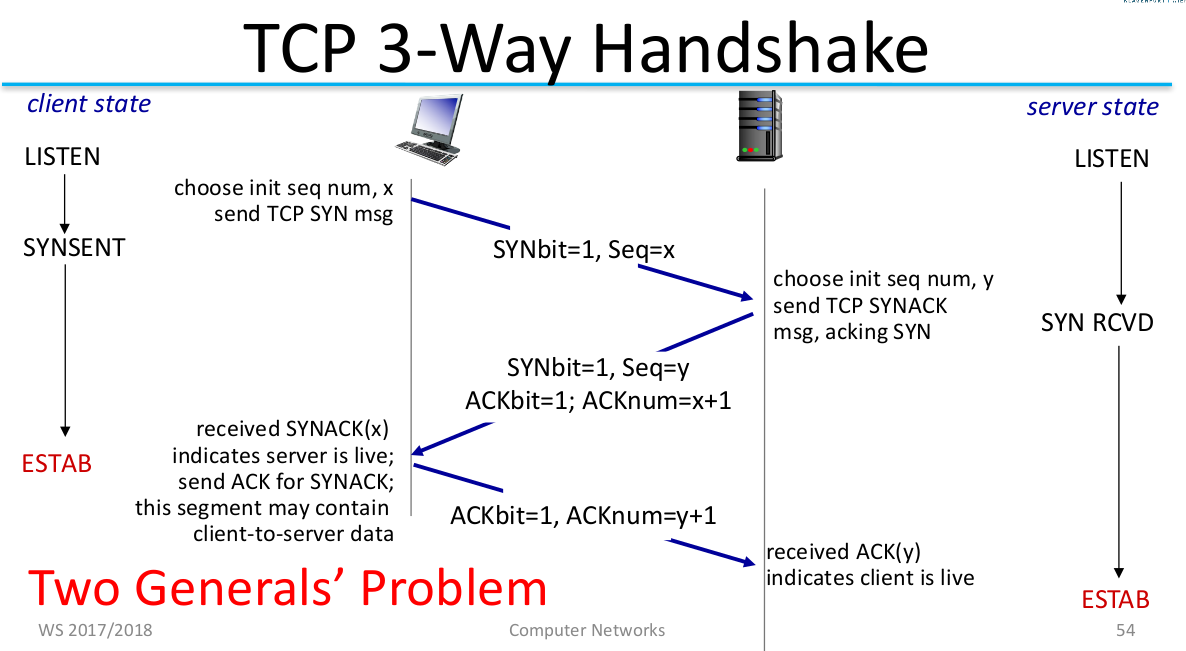
\includegraphics[width=\textwidth]{TCPHandshake.png}
    \end{center}
        
        Der Abbau geschieht mittels der FIN-Flag. Sobald der Klient die Verbindung schließen möchte, 
        so wird die FIN-Flag gesetzt, 
        wodurch der Client keiner weiteren Daten schicken darf, jedoch noch empfangen kann. 
        Die Verbindung ist dann abgebaut, wenn ein Klientseitiger Timer ausläuft oder die FIN-Flag seitens Server eintrifft.\\
        \begin{center}
            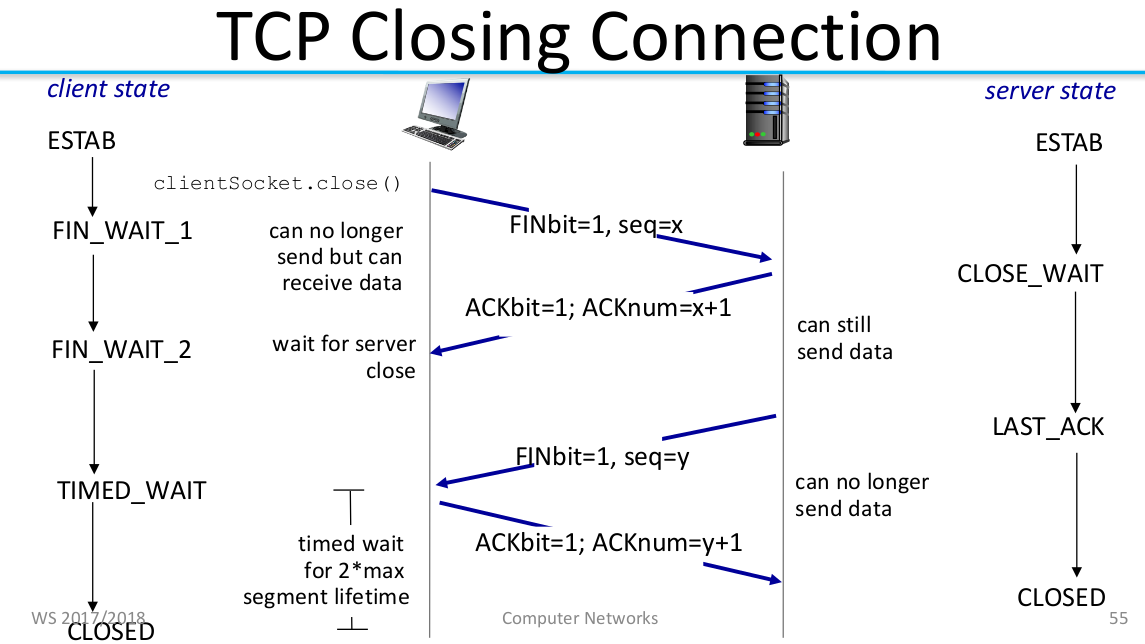
\includegraphics[width=\textwidth]{TCPShutdown.png}
        \end{center}
        
        \item \textbf{Netzwerkschicht}:
        Nenne und beschreibe die drei Hauptfunktionen der Netzwerkschicht und nenne die zwei bekanntesten Routingalgorithmen.
        Die Netzwerkschicht, oder Networklayer, dient dem Forwarding, dem Routing und der Fragmentierung der Datenpakete in Frames.
        
        \begin{description}
            \item [Forwarding] How each router makes the decision as to where to send a packet next is called the \textbf{forwarding algorithm}.
            \item [Routing] How the network makes the decision as to which path to use is called the \textbf{routing algorithm}.
        \end{description}
        
        Zu den bekannten Routingalgorithmen zählen der \textbf{Dijkstra-Algorithmus oder Link State} und der \textbf{Distance-Vector}.
        
        \item \textbf{Netzwerkschicht}: Beschreibe IPv4 bzw. IPv6 und gehe auf Unterschiede ein und skizziere mögliche Ansätze zum Übergang von IPv4 und IPv6.
        IPv4 als auch IPv6 spezifiziert jedes Gerät anhand einer eindeutigen Adresse im jeweiligen Subnets.
        
    Während IPv4 einen Adressbereich von $2^{32}$, oder $256^{4}$, bietet, 
    so bietet IPv6 einen Adressbereich von $2^{128}$. 
    IPv6 ist üblicherweise codiert in Hexdadezimalzahlen, wobei einzelne Blöcke mittels ':' getrennt werden.
    
        \begin{verbatim}
https://213.213.220.07/                         -- IPv4
http://[2001:0db8:85a3:08d3::0370:7344]/        -- IPv6
http://[2001:0db8:85a3:08d3::0370:7344]:8080/   -- IPV6 + Port
        \end{verbatim}
        
        IPv4 Adressen werden in 4 verschiedene Klassen eingeteilt (Heuertags eigentlich Klassenlos berechnet):
        \begin{enumerate}
            \item Klasse A: 8 Bit-Netz \& 24 Bit Host-Adresse 
            \item Klasse B: 16 Bit-Netz \& 16 Bit Host-Adresse
            \item Klasse C: 24 Bit-Netz \& 8 Bit Host-Adresse
            \item Klasse D: 28 Bit-Multicastgruppen
    \end{enumerate}
        Die zu vergebenden Hostadressen berechnet sich mit $2^{Anzahl an Bits für Hostadresse} - 2$. 
        Dabei sind spezifische Adressen stets reserviert: 192.168.0.0/8 ist das Netzwerk selbst, 
        während 192.168.0.255/32 ist der Broadcast innerhalb dieses Netzes.
        
        IPv4 -- Klasse C-Netzberechnung:\\
        Bei einem Subnetz von 11111111.11111111.11111111.00000000 (255.255.255.0) wird der Netzteil auf 192.168.0 festgelegt $\leftrightarrow$ E.g. wir besitzen 8 Bits für unsere Hostadressen.\\
        $\rightarrow$ Der Netzname ist predefiniert mit .0\\
        $\rightarrow$ Der Broadcsat liegt auf .255\\
        $\rightarrow$ Wir können damit noch $2^8 - 2$ Adressen belegen, dementsprechend hat dieses Netz noch 254 Adressen zur Verfügung.\\
        
        Dies funktioniert analog mit dem Klassenlosen IPv4 Verteilungsprinzip, bei welchem man die höchstwertigen Bits (von Links) dem Netzteil zuspricht. Der Rest resolviert die Anzahl an zu vergebene Adressen.\\
        Für einen Netzteil von 192.168.120 $\leftrightarrow$ 11000000.10101000.01111 existiert ein möglicher Host-Adressbereich von $32-8-8-5 = 11$ setzbaren Bits, dementsprechend haben wir $2^11 - 2 = 2046$  Adressen. \\
        
        IPv6 -- Adressberechnung\\
        .. verläuft nach demselben Schema wie bei IPv4. Die Adressen werden in ihre Bits transformiert und es werden Netz- und Hostadressbereiche eingeteilt.
        Der Wert nach einer IPv6 Adresse (.../12) beschreibt die Anzahl der Bits für den Netzanteil. Der Rest der Adresse beschreibt den Hostanteil. 
        \begin{center}
            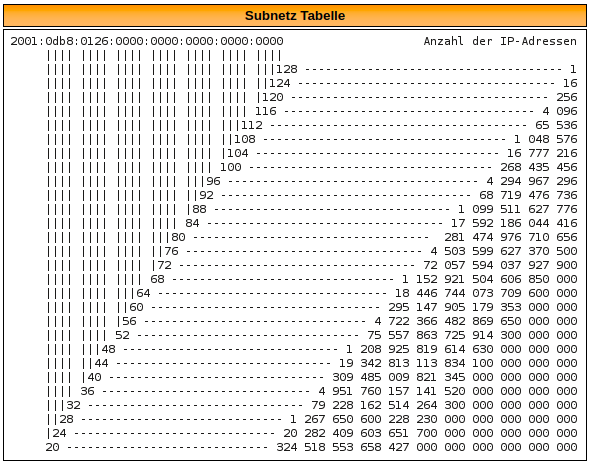
\includegraphics[width=\textwidth]{IPv6Subnetze.png}
        \end{center}
        
        \item \textbf{Sicherungsschicht}: Beschreibe CSMA/CD und CSMA/CA. Wo werden die Methoden eingesetzt?
        \item \textbf{Sicherungsschicht}: Beschreibe ARP.
        \item \textbf{Rechnernetze Allgemein}: Beschreibe die Funktionsweise und Unterschiede von paketvermittelnden und leitungsgebundenen Netzwerken?
    \end{enumerate}
    \subsection{Frei erfundene Bsp.}
    \subsubsection{Theorie}
    \begin{enumerate}
        \item Ordne folgende Protokolle den Schichten des TCP-Modelles zu:
        \begin{center}
            \begin{tabular}{l|lll|l}
                SMNP        & $\bullet$ & & $\bullet$ &  Anwendungsschicht   \\
                POP3        & $\bullet$ & & $\bullet$ &  Transportschicht    \\
                ARP         & $\bullet$ & & $\bullet$ &  Vermittlungsschicht \\
                DNS         & $\bullet$ & & $\bullet$ &  Netzzugangsschicht  \\
                TLS         & $\bullet$ & & $\bullet$ &                      \\
            \end{tabular}
        \end{center}
        \item Was ist der Unterschied zwischen Flow Control und Congestion Control?
        \item Was sind die unterschiedlichen Elemente eines Wireless Networks und wie arbeiten sie miteinander?
        \item Was passiert wenn man innerhalb eines WLan-Netzwerkes den Standort wechselt? 
        \item Was sind die 5 Eckpfeiler des 5G Atoms und welche Teilbereiche gibt es?
        \item Was bedeutet ''Multiple Access'' im Rahmen des IEEE 802.11?
        \item Was sind nennenswerte Unterschiede zwischen ARP und DNS?
        \item Worin unterscheiden sich Router und Switches?
        \item Wie funktioniert der Link Layer und was ermöglicht dieser? Skizziere!
        \item Wie unterscheiden sich TDMA, FDMA, CDMA? Skizziere.
        \item Wie funktioniert BGP? Gibt es äquivalente Protokolle?
        \item Welche Arten der Datenübertragungen gibt es und welche grundlegenden Protokolle werden dafür implementiert? 
        \textit{Tip: Uni-Cast sendet von 1 zu 1 weiterem.}
        \item Wie funktioniert SDN?
        \item Was sind Grundfunktionalitäten der Applikationsschciht. Welche Protokolle werden hier implementiert?
        \item Wie unterscheiden sich Data Plane und Control Plane? Gibt es unterschiedliche Variationen des Control Plane?
        \item Wie wird ein IPv6 Paket behandelt, sollte man lediglich IPv4 weitersenden können?
        \item Welche Versionen von HTTP existieren und was sind Unterschiede zwischen den einzelnen Versionstypen? Ist HTTP ein sicheres Protokoll?
    \end{enumerate}
    \subsubsection{Berechnungen}
    \begin{enumerate}
        \item I seriously fucking hope this wont come.
        \item Welche Arten der IP-Adressierungen gibt es? Wie werden Geräte adressiert? % Add bsp
    \end{enumerate}
    \subsubsection{Wahr oder Falsch}
    \begin{enumerate}
        \item IEEE 802.11 ist ein Transportprotokoll.
        \item Mithilfe der Datenrate-adaption kann man Datenqualität optimieren. Das SNR verstärkt diese Optimierung.
        \item DAS SNR ist eine relative Maßzahl von Geräusch und Signal. Je höher das SNR, desto schlechter ist es.
        \item Die Verarbeitung der MAC Addresse gehört zur Vermittlungsschicht
        \item Das 802.3 ist eine veraltete Version des 802.11.
        \item Der Link Layer wird abstrahiert in 2 Unterebenen, Dataplane und Controlplane.
        \item P2P-Protokolle, also PPPs, verwenden Switches zur Übertragung.\\
        
        
        \item TDMA und FDMA sind zeitlich gesehen gleich schnell mit Datenübertragungen.\\
        Prinzipiell Ja. Wir betrachten zunächst beide Implementierungsmöglichkeiten:
        \begin{center}
            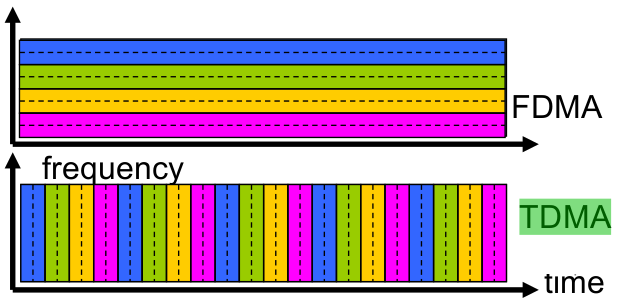
\includegraphics[width=0.8\textwidth]{TDMAvsFDMA.png}
        \end{center}
        Der einzige Unterschied zwischen FDMA und TDMA ist dessen Platzkomplexität. FDMA benötigt mehr Frequenzen, wodurch das System, per User, außerordentlich groß sein muss.
        TDMA kann auf einem einzigen Kanal mehrere User unterhalten, jedoch auf Kosten der Qualität.
        Siehe auch: 
        \begin{verbatim}
        https://www.taitradioacademy.com/topic/the-difference-between-fdma-and-tdma-1/
        \end{verbatim}
        
        \item Die Abkürzung 'AS' steht für ''automated Services'' und steht im Zusammenhang mit Routerregionen.\\
        Falsch, AS steht für 'Autonomous System'. Diese jedoch stehen tatsächlich in Zusammenhang mit Routerregionen.
        
        \item BGP dient dem Forwarding von Paketen.\\
        Richtig, wobei es allgemein den Pakettransit, durch Ermitteln des nächst-günstigsten Nachbars, unterstützt.
        
        \item Bei ''Multicast'' sendet genau 1 Sender an beliebig viele Empfänger.\\
        Richtig. Normalerweise mittels UDP.
        .
        \item SDN implementiert Congestion Control.\\
        Falsch, SDN implementiert lediglich Flow-based forwarding. Es gibt jedoch eine Erweiterung, das SDTCP, welches Congestion control implementiert. 
        
        \item Es ist möglich mittels SNMP auf Geräte im gleichen Netzwerk zuzugreifen.\\
        Richtig, man erinnere sich an Timmse's Präsentation des SNMP auf Druckerzugriff im Rahmen der x'ten LV-Einheit. Anhand verschiedenen Befehlen kann man Geräte direkt ansprechen, soweit man im gleichen Netzwerk ist. Jedoch muss man dies per Gerät freigeben.
        
        \item Die Begriffe ''Openflow'' und ''Flooding'' beschreiben exakt das gleiche.\\
        Falsch, Flooding beschreibt den Vorgang, in welchem ein Router alle unterliegenden Geräte abfragt (ähnlich wie Broadcast). Openflow ist Teil des SDN als Kommunikationsprotokoll. Es gibt Zugriff auf Hardwarekomponente des Switches oder ROuters zur Bearbeitung eintreffender Netzwerkpakete (Auch \textit{Forwarding Plane} genannt).
        
        \item Die Firewall, etwa im OpenFlow, vergleicht IP-Adressen und TCP/UDP Port Nummern. Anhand dessen werden Daten akzeptiert oder gesperrt.\\
        Richtig.
        
        \item Forwarding ist ein äquivalenter Ausdruck für Routing.\\
        Nein. Forwarding beschreibt wohin ein Packet gesendet wird, während Routing die Route betrachtet, welche das Packet vom Sender zu Empfänger hintergelegt hat.
        
        \item Das Hot Potatoe Routing nutzt Flooding zur Datenweitergabe.\\
        Falsch. Anhand iBGP wird bereits vornherein ermittelt, wer der nächst-günstigste Nachbar zum übertragen ist. Zu diesem wird dann gesendet.
        
        \item Der Networklayer implementiert die Funktionen des Forwarding und des Routing.\\
        Falsch, das wird von der Vermittlungsschicht übernommen. Der Netzworklayer dient dem Zustellen zur richtigen MAC-Addresse
        
        
        \item Eine IPv4-Addresse deckt einen Adressbereich von $2^(32)$ Addressen ab.\\
        Richtig, wobei viele davon vorreserviert sind, wie etwa 255.255.255.255 (Broadcast). 
        % TODO: Actually check this, but should fit
        
        \item Jeder einzelne Router, welche ein Paket durchläuft, prüft die Checksumme des Paketes auf dessen Richtigkeit.\\
        Richtig. Bei Verwurf des Paketes wird auch kein neues angefordert.
        Alternativ, wenn die Time-To-Life ausläuft wird es ebenso verworfen.
        
        \item IPv6 und IPv4 unterscheiden sich lediglich durch Header, welche in IPv6 neu implementiert wurden: Priority, Flow Label und Next Header-Field.\\
        Falsch, es gibt weitere Felder die geändert wurden.
        
        \begin{verbatim}
        IPv4 Header-felder:
         0                   1                   2                   3
         0 1 2 3 4 5 6 7 8 9 0 1 2 3 4 5 6 7 8 9 0 1 2 3 4 5 6 7 8 9 0 1
        +-+-+-+-+-+-+-+-+-+-+-+-+-+-+-+-+-+-+-+-+-+-+-+-+-+-+-+-+-+-+-+-+
        |Version|  IHL  |Type of Service|          Total Length         |
        +-+-+-+-+-+-+-+-+-+-+-+-+-+-+-+-+-+-+-+-+-+-+-+-+-+-+-+-+-+-+-+-+
        |         Identification        |Flags|      Fragment Offset    |
        +-+-+-+-+-+-+-+-+-+-+-+-+-+-+-+-+-+-+-+-+-+-+-+-+-+-+-+-+-+-+-+-+
        |  Time to Live |    Protocol   |         Header Checksum       |
        +-+-+-+-+-+-+-+-+-+-+-+-+-+-+-+-+-+-+-+-+-+-+-+-+-+-+-+-+-+-+-+-+
        |                       Source Address                          |
        +-+-+-+-+-+-+-+-+-+-+-+-+-+-+-+-+-+-+-+-+-+-+-+-+-+-+-+-+-+-+-+-+
        |                    Destination Address                        |
        +-+-+-+-+-+-+-+-+-+-+-+-+-+-+-+-+-+-+-+-+-+-+-+-+-+-+-+-+-+-+-+-+
        |                    Options                    |    Padding    |
        +-+-+-+-+-+-+-+-+-+-+-+-+-+-+-+-+-+-+-+-+-+-+-+-+-+-+-+-+-+-+-+-+
        \end{verbatim}
        
        \begin{verbatim}
        IPv6 Header-Felder:
         0                   1                   2                   3
         0 1 2 3 4 5 6 7 8 9 0 1 2 3 4 5 6 7 8 9 0 1 2 3 4 5 6 7 8 9 0 1
        +-+-+-+-+-+-+-+-+-+-+-+-+-+-+-+-+-+-+-+-+-+-+-+-+-+-+-+-+-+-+-+-+
        |Version| Traffic Class |           Flow Label                  |
        +-+-+-+-+-+-+-+-+-+-+-+-+-+-+-+-+-+-+-+-+-+-+-+-+-+-+-+-+-+-+-+-+
        |         Payload Length        |  Next Header  |   Hop Limit   |
        +-+-+-+-+-+-+-+-+-+-+-+-+-+-+-+-+-+-+-+-+-+-+-+-+-+-+-+-+-+-+-+-+
        |                                                               |
        +                                                               +
        |                                                               |
        +                         Source Address                        +
        |                                                               |
        +                                                               +
        |                                                               |
        +-+-+-+-+-+-+-+-+-+-+-+-+-+-+-+-+-+-+-+-+-+-+-+-+-+-+-+-+-+-+-+-+
        |                                                               |
        +                                                               +
        |                                                               |
        +                      Destination Address                      +
        |                                                               |
        +                                                               +
        |                                                               |
        +-+-+-+-+-+-+-+-+-+-+-+-+-+-+-+-+-+-+-+-+-+-+-+-+-+-+-+-+-+-+-+-+
        \end{verbatim}
        
        \item TCP implementiert Multicast.\\
        Falsch, TCP ist ein direktes P2P Protokoll. Multicast wird mittels UDP implementiert, aufgrund des Abysmalen Overheads des TCP.
        
        \item Existieren Bitfehler in einem Datenpaket, so können diese mithilfe der Checksumme erkannt werden.\\
        Richtig, die Checksumme wird in jedem Router neuberechnet.
        
        \item Bei Selective Repeat existieren Fehlermöglichkeiten, welche den Algorithmus außer Kraft setzen.\\
        Ja, es gibt die Möglichkeit dass bei ACK-Verlust die Synchronisation von Klient und Server flöten geht.
        \begin{center}
            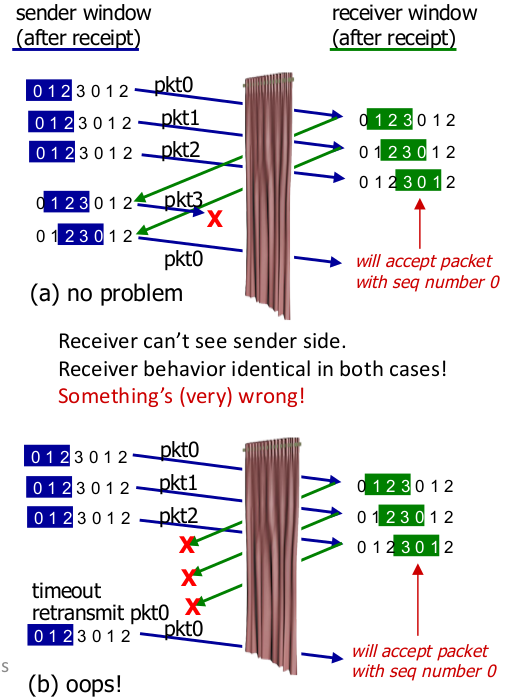
\includegraphics[width=\textwidth]{SelectiveRepeat_Error.png}
        \end{center}
        
        \item Für Go-Back-N gilt: Es wird solange das gesamte Window neugesendet, bis die ACKs aller Pakete empfangen wurden.\\
        Falsch. Es werden lediglich die Pakete gesendet, welche keine ACK zurücklieferten. Anschließend wird das Window nach vorne verschoben.
        Siehe: 
        \begin{verbatim}
http://www.ccs-labs.org/teaching/rn/animations/gbn_sr/
        \end{verbatim}
        
        \item Die Abfrage von IP-Adressen mittels DNS ist sowohl rekursiv als auch iterativ ausführbar.\\
        Wahr. 
        
        \item Aufgerufene Adressen werden werden im Schnitt für 2 Tage gecached.\\
        Wahr, wobei diese Zeit konfiguierbar ist.
        
        \item HTTP-Fehlercodes beginnend mit 5 beschreiben Klient-Fehler.\\
        Falsch, dies sind Server-Fehler. Klient-Fehler sind 4xx.
        \end{enumerate}
        
\section{Sources}
    \begin{verbatim}
- https://www.elektronik-kompendium.de/sites/net/0503281.html
- http://www.ipv6-portal.de/tools/subnet-tabelle.html
- https://talvindersingh1992.wordpress.com/2013/07/07/multiple-access-techniques-tdma-fdma-cdma/
- VO-Folien
- Wikipedia
    \end{verbatim}



\end{document}

